\documentclass[10pt]{article}
\usepackage[tmargin=1.25in,lmargin=1in,rmargin=1in,bmargin=1in,paper=letterpaper]{geometry}
\usepackage{amsmath,amssymb,amsthm}
\usepackage{multirow,color}
\usepackage{fancyhdr,ifthen,lastpage}
\usepackage{relsize,changepage}
\usepackage{enumitem,empheq,float,caption}
\usepackage{listings}
\usepackage{tikz,tikz-qtree,tikz-qtree-compat}
\usetikzlibrary{shapes,backgrounds,calc,patterns,snakes,angles,quotes}
\usepackage{hyperref}
\usepackage{mathtools}
\usepackage{framed}
\usepackage{chessboard}
\usepackage{skak}
\usepackage[normalem]{ulem}
\usepackage[hang,flushmargin]{footmisc}
\usepackage{textcomp}
\usepackage{pifont}
\newcommand{\cmark}{\ding{51}}%
\newcommand{\xmark}{\ding{55}}
\usepackage{fix-cm}
% --------------------------------------------------------------------
\renewenvironment{leftbar}[1][\hsize]
{%
    \def\FrameCommand
    {%
        {\color{black}\vrule width 1.5pt}%
        \hspace{7pt}%%
        \fboxsep=\FrameSep%
    }%
    \MakeFramed{\hsize#1\advance\hsize-\width\FrameRestore}%
}%
{\endMakeFramed}
\newenvironment{leftbara}[1][\hsize]
{%
    \def\FrameCommand
    {%
        {\color{gray}\vrule width 1.5pt}%
        \hspace{7pt}%
        \fboxsep=\FrameSep%
    }%
    \MakeFramed{\hsize#1\advance\hsize-\width\FrameRestore}%
}%
{\endMakeFramed}
\newcommand\irregularcircle[2]{% radius, irregularity
  let \n1 = {(#1)+rand*(#2)} in
  +(0:\n1)
  \foreach \a in {10,20,...,350}{
    let \n1 = {(#1)+rand*(#2)} in
    -- +(\a:\n1)
  } -- cycle
}
\newcommand{\cvdots}[1][=]{\mathrel{\makebox[\widthof{#1}]{\vdots}}}
\DeclareMathOperator*{\bigplus}{\text{\fontsize{25}{35}\selectfont $+$}}
\DeclareMathOperator*{\bigtimes}{\text{\fontsize{25}{35}\selectfont $\times$}}

% --------------------------------------------------------------------
\newcommand{\isdef}{\stackrel{\mathrm{def}}{=}}
\def\multiset#1#2{\ensuremath{\left(\kern-.3em\left(\genfrac{}{}{0pt}{}{#1}{#2}\right)\kern-.3em\right)}}
\newcommand\RR{{\mathbb R}}
\newcommand\QQ{{\mathbb Q}}
\newcommand\CC{{\mathbb C}}
\newcommand\ZZ{{\mathbb Z}}
\newcommand\NN{{\mathbb N}}
\renewcommand\mod{{\text{ mod }}}
% --------------------------------------------------------------------
\newtheorem{theorema}{Theorem}[section]
\newtheorem{corollarya}{Corollary}[theorema]
\newtheorem{lemmaa}[theorema]{Lemma}
\newtheorem*{remark}{Remark}
\theoremstyle{definition}
\newtheorem{axioma}{Axiom}
\newtheorem{definitiona}{Definition}[section]
\newtheorem{sketcha}{Sketch}[section]
\newtheorem{techniquea}{Technique}
\newtheorem{scholium}{Scholium}
\newtheorem{example}{Example}[section]
\renewcommand\qedsymbol{$\blacksquare$}
% \newenvironment{definition}
%     {\pushQED{\qed}\renewcommand{\qedsymbol}{$\triangle$}\examplex}{\popQED\endexamplex}
\let\olddef\definition
\newenvironment{definition}{\begin{leftbar}[.95\linewidth]\begin{definitiona}}{\end{definitiona}\end{leftbar}}
\newenvironment{theorem}{\begin{leftbar}[.95\linewidth]\begin{theorema}}{\end{theorema}\end{leftbar}}
\newenvironment{lemma}{\begin{leftbar}[.95\linewidth]\begin{lemmaa}}{\end{lemmaa}\end{leftbar}}
\newenvironment{corollary}{\begin{leftbar}[.95\linewidth]\begin{corollarya}}{\end{corollarya}\end{leftbar}}
\newenvironment{axiom}{\begin{leftbar}[.95\linewidth]\begin{axioma}}{\end{axioma}\end{leftbar}}
\newenvironment{sketch}{\begin{leftbara}[.95\linewidth]\begin{sketcha}}{\end{sketcha}\end{leftbara}}
\newenvironment{technique}{\begin{leftbara}[.95\linewidth]\begin{techniquea}}{\end{techniquea}\end{leftbara}}
\usepackage{cancel}

\newcommand{\abs}[1]{\left| #1 \right\|}
\newcommand{\set}[1]{\left\{ #1 \right\}}
\newcommand{\mylist}[1]{\left( #1 \right)}

\let\oldref\ref
\renewcommand{\ref}[1]{(\oldref{#1})}

\begin{document}
\pagestyle{fancy}

\setlength{\headheight}{0pt}
\setlength\parindent{0pt}

\lhead{ Math 30B -- Fall 2016}
\rhead{Forest Kobayashi}
\chead{\bf Calculus Notes}


\setlength{\headheight}{0pt}
\tableofcontents
% ========================================================================
\newpage
\section{Preface}
\subsection{What is math?}
I have been frustrated for quite some time with how mathematics is taught to most students.  Oftentimes, classes take one of the following approaches to teaching mathematics:
\begin{enumerate}
    \item `\textbf{Math is all about numbers and computation.}'  Here, mathematics is typically described as (and thus, usually understood by students to be) a \emph{tool}, or some sort of useful \emph{skill}.  In this sense, math is taught as a means to an end that can be employed to answer important questions about the real world.  Frequently, such courses focus more on covering a wide range of topics (for the purpose of teaching students many different applicable scenarios) than they do on giving students a foundational understanding of the topic.  
    \item `\textbf{Math is all about rigor.}'  In these classes, students are led to believe that memorizing notational standards, being as pedantic as possible, and employing exactingly literal statements in definitions / proofs are what constitute `real' mathematics.  This reliance on rigor can often lead to what Terence Tao describes as `compile errors,' in which a slight ambiguity in a definition or theorem statement creates an `impass' of sorts that the reader cannot continue past.
\end{enumerate}
Now, I don't mean to imply that mathematics involves neither of these things---certainly (to some degree or another) almost all fields of  mathematics require the occasional encounter with numbers, and (occasionally oppressive) doses of rigor with which to support one's claims.  My issue lies in the fact that people percieve these to be \emph{all there is} to math, or as what math (in some sense) fundamentally \emph{is}.\\~\\
I once heard a quote that I think encapsulates this idea nicely: `Mathematics is no more about numbers than a poem is about letters.'  Sure, mathematical ideas are often \emph{reflected} in numbers (or other mathematical objects)---but they don't constitute the \emph{heart} of mathematics.  That, generally speaking, lies instead in the particular \emph{pattern} or \emph{concept} under discussion.  In this sense, I think it is most accurate to describe math as the study of \textbf{structure}.  \\~\\
Many people who bemoan the focus math classes place on computation and rigor will tell you that what math is \emph{really} about is \textbf{problem-solving}, and learning the associated skills.  I think that this too somewhat misses the point, for two reasons.  First, `problem-solving' to me implies a sense in which a solution is the \emph{end goal} of mathematics.  In that sense, it implies that after finishing a proof or getting the same number that's in an answer key, we can move on with our lives and forget about what we've just shown.  And furthermore, it implies that if we \emph{don't} get the same answer (or just can't \emph{quite} piece together a cohesive proof), that we have `failed' in some sense.  I do not think these is really the case---ultimately, a lot of `mathematics' comes in the form of looking back over a solution, and trying to tease out deeper understandings of \emph{why} it worked (or didn't), and what kind of futher understandng we can glean from it.  And second, the word `solution' seems to imply some sort of linearity, or standardization to the method by which we reached it.  But in mathematics (at least, past the foundational material we'll be covering in the chapters of this document), this frequently not the case.  In fact, there are sometimes \emph{many} different possible solution methods for a given problem, each of them equally valid!  In this sense, lots of mathematical problem-solving comes in the form of trying to look at a single idea from many different perspectives, instead of just trying to find a single one that works.  \\~\\
%As evidence, I point to the fact that I am still interested in mathematics.  I mean, if I thought math were about problem \emph{solving}, I'd have quit long ago!  After all, if I cared about getting \emph{solutions}, why would I continue to spend 5 hours on a single math problem without making \emph{any} headway towards a solution, when I could find `solutions' to tens (or even hundreds) of physics problems in the same amount of time?  And besides, if math were all about problem-solving, where would proofs fit into it?  In being asked to \emph{prove} a statement, aren't we being given a `solution' before we even begin?  \\~\\
% Sure, you could argue that in our case, the \emph{proof} is the `solution' to the `problem' we've been given, which is `how can we show \underline{\quad\quad}?'  But I think the word \emph{solution} implies some degree of uniqueness, or standardization---i.e., that if something is the `solution' to a problem, it is (in some sense) the `way things should be done.'  And, although this is typically the way mathematics is taught, it couldn't be further from the truth.  As long as you reach the same end point, \\~\\should not be although most math classes (and even this document) involve countless pages of `exercises' and `practice problems,' I think that saying math is about `problem solving' misses the point as well.  \\~\\
There's one very important part of mathematics that I have so far neglected to discuss: the issue of \emph{communication}.  This is about equally important as everything listed above: 
% So, to summarize, here's \emph{my} view on what math `is', math is primarily concerned with two things:
% \begin{enumerate}
% \item 
% \end{enumerate}

%  Calculus is delivered to students in one of two ways:
% \begin{enumerate}
%     \item With a computational focus.  In these classes, derivatives and integrals are typically taught as a bunch of formulae to be memorized and then employed to solve some uninspiring example problems.  Usually, a teacher will use derivations and proofs as a means to an end
%     \item 
% \end{enumerate}
\subsection{About this document, and how to read it}
% \subsection{A brief overview of some common notations}
% \subsection{Logic (Optional)}
\clearpage
\section{Sets \& Induction}
\subsection{Sets}
\subsubsection{Definition of a Set}
We first discuss the definition of a \emph{set}.  Set theory is the language of mathematics, so it is important to have a foundational understanding of sets before continuing onto more advanced topics.  Most of the grammar/syntax for sets is fairly simple, but can take us a surprisingly long way towards understanding more abstract mathematical concepts.  So what is a set?  In a loose sense, a set is just a collection of distinct objects.  A hand of cards is a set, a straight line is a set of points on that line, an album is a set of songs, etc.  More formally, a set is defined as
\begin{definition}[Set]
A \textbf{set} is an unordered collection of objects (called \textbf{elements}) in which repetition doesn't matter.  We typically write a set as
\[\text{Set} = \set{\text{element 1},~\text{element 2},~\text{element 3},~\ldots}\]
read as `the set containing element 1, element 2, element 3, $\ldots$'  Typically, we denote a set with a capital letter (e.g., `the set $S$'), and its elements with a lower-case letter. 
\end{definition}
There're a lot of subtleties to this definition, so let's break it down piece by piece.  First, a set is a \emph{collection} of objects---even if it has just one element (or, even if it has \emph{no} elements at all---it still counts as a `collection,' just an empty one)!  Thus, the set $\set{a}$ is \emph{not} the same thing as the element $a$.   
\[a \neq \set{a}\]
As a contrived example, we can think of this difference as being the same distinction we draw between a committee comprised of one person and that person themself, or the difference between a class consisting of one student and that student themself.\footnote{this taken from Maxwell Rosenlicht's \textit{Introduction to Analysis}}  The `unordered' portion of our definition means that it doesn't matter what order we choose to list the elements of the set in; all that matters is what the elements of the set are.  As an example, the sets 
\begin{align*}
S_0 &= \set{1,2,3}\\
S_1 &= \set{3,1,2}
\end{align*}
Are `the same' even though they look different from one another, because both contain 1, 2, 3, and no other elements.  A more tangible real-world example of this is a hand of cards---in most flavors of poker, the hands
\begin{align*}
H_0 &= \set{10\clubsuit,9\clubsuit, 8\clubsuit, 7\clubsuit, 6\clubsuit}\\
H_1 &= \set{7\clubsuit,9\clubsuit, 10\clubsuit, 6\clubsuit, 8\clubsuit}
\end{align*}
would be considered to be the same straight flush, because all that matters is \emph{what} cards we have, not what order they're in.  The `repetition doesn't matter' portion of our definition means that a set such as
\[S_2 = \set{1,1,1,1,3,2}\] 
Is also `the same' as $S_0$ and $S_1$.  This is because all that is important when discussing a set is \emph{what} is in the set, not \emph{how many times} we assert it is in the set.\footnote{If we were to read out our description of $S_2$, it would be `the set that contains 1, contains 1, contains 1, contains 1, contains 3, and contains 2.'  The second, third, and fourth times we say `contains 1' are each redundant, because each one only tells us our set contains 1, which has already been asserted by the first.}  So, the fact that we wrote $S_2$ with four 1's doesn't actually make it distinct from $S_0$ and $S_1$.  
\\
Another property of sets is that they can have \emph{any} number of elements.  For instance, the set containing no elements (also referred to as the `null set') is given by 
\[\varnothing = \set{}\]
Where $\varnothing$ is a fancy shorthand we use to refer to the null set, because it comes up a lot in mathematics.\footnote{I don't think this will pop up anywhere in my notes here, but the `size' of a set (or more accurately, a measure of the number of elements it contains) is called the `cardinality' of the set, and is denoted with vertical bars (like absolute value symbols).  E.g., $|\varnothing| = 0$, because $\varnothing$ has 0 elements.}  
Elements of a set can be pretty much anything, not just numbers (we can even have sets of sets!).  For instance, we can consider the set of Philosophers who aren't totally full of crap (denoted $P$): 
\[P = \varnothing\]
In mathematics, we have a special notation for `is in the set', which we denote by $\in$.  This is also read as `is an element of,'\footnote{which, I imagine, is probably where the notation for $\in$ looking kind of like a weird E comes from} with the element in question on the left hand side of the $\in$, and the set on the right hand side.  We can also say something is \emph{not} an element of a set, and this is denoted by $\notin$.  For instance, 
\begin{align*}
1&\in\set{3,1,8}\\
2&\notin\set{3,1,8}
\end{align*}
Some more mathematical shorthand: $\forall$ means `for all,' and we can use it to say something that applies to all elements of a set.  As an example, we might have
\[\forall x\in \set{0,1,2,3}, x\geq 0\]
which is read as `for all $x$ in the set ${0,1,2,3}$, $x$ is greater than or equal to zero (or, $x$ is non-negative).'  Another important symbol is $\exists$, which means `there exists.'  This is usually coupled with $:$ or $|$, which are two different notations for saying `such that.'  I'll try to stick to $:$ for `such that' in these notes (because $|$ is used as `divides' elsewhere in mathematics), but if you spot what you think might be an error, please let me know!  Here's an example of all of these symbols working in conjunction:
\[\exists x\in \set{0,1,2,3} : \forall y\in\set{0,1,2,3},~x\leq y\]
This general readability of this statement is quite low, so let's break it down piece by piece.  The part before the $:$ is telling us that there is (i.e., there exists) some $x$ in the set $\set{0,1,2,3}$ that satisfies the conditions that we will find on the right hand side of the $:$.  The part to the right of the $:$ tells us the properties of this $x$---namely, that $x$ is \emph{at least} as small as every element $y$ in the set $\set{0,1,2,3}$.  But, this is the same set we took $x$ from, so we can reword our statement as ``there is some element of $\set{0,1,2,3}$ that is smaller than or equal to every other element in the set $\set{0,1,2,3}$, including itself.''  Or, even more succinctly, `the set $\set{0,1,2,3}$ has a least element.'  \\~\\
You might be thinking `Man, the verbal description in the line above seems a lot clearer than the opaque symbols we used at first.  But, I'm guessing there's some abstract advantage to using the math-y notation instead of plain English, because it certainly looks imposing and therefore must carry more rhetorical/logical heft.  Is that it?'  Well, I'm glad \sout{you} I asked!  I think the answer is basically, `No, not really.'  Here, the plain English description simply does a better job of describing what's going on than our symbol-heavy explanation does, even though it contains a `judicious' amount of rigor\texttrademark and quantifiers.\footnote{`Quantifiers' are what things like the $\forall$ and $\exists$ symbols are called}  \\~\\
Now, that doesn't mean that things like $\forall$ and $\exists$ are useless---in fact, they can often be the better choice of notation.  For instance, when dealing with complicated expressions, they can help declutter the page (thus making the flow of reasoning easier to follow), and sometimes just working in the more `abstract' mathematical language can make it easier to obtain insight.  But make no mistake: the first statement (the one with symbols) isn't any more `mathematical' than the second one; if anything, I would actually argue the first is \emph{less} mathematical, because it does a poor job of communicating what should be a simple idea to a reader.  Ultimately, mathematics should be about clarity and insight, and communicating something simple to a reader, not about dense notation that looks pretty.  
\begin{figure}[H]
\centering
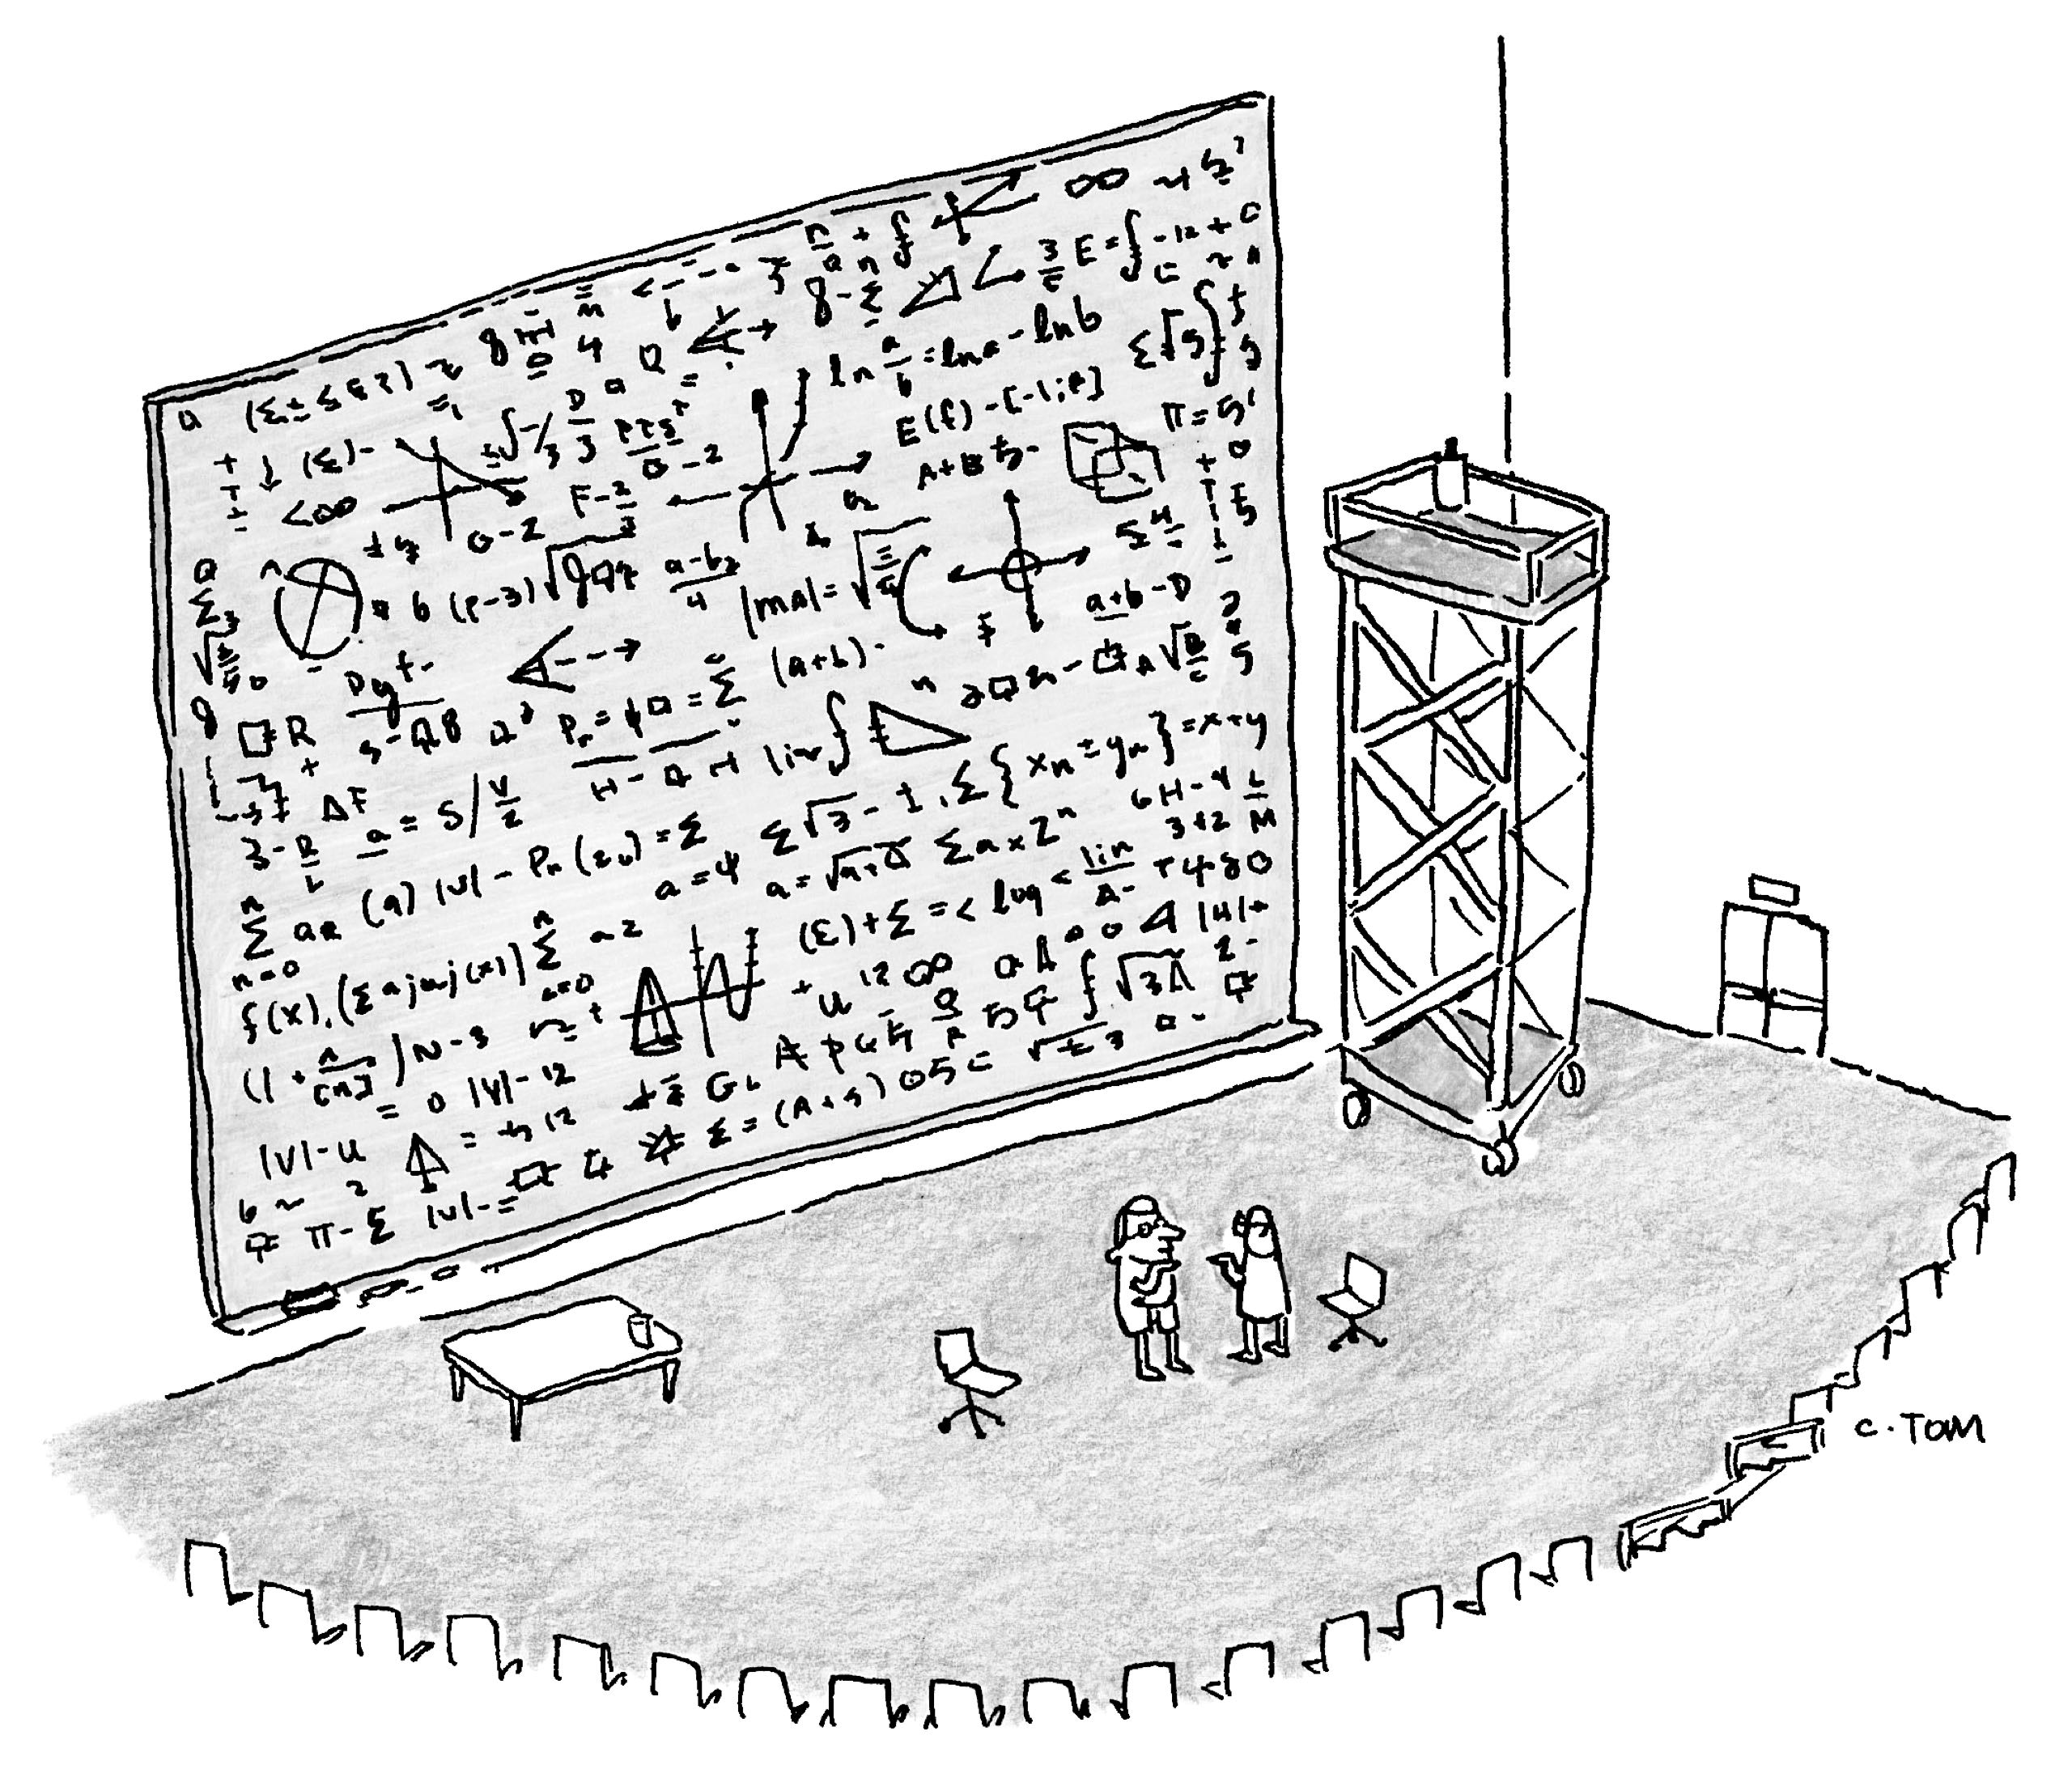
\includegraphics[width=10cm]{math.jpg}
\caption*{``The math is right. It’s just in poor taste.'' Source: The New Yorker}
\end{figure}
Before moving onto the next section, I think it's worth mentioning that the example I gave is actually a specific case of an \textbf{axiom} that will become important to us later, called the \textbf{Well-Ordering Principle} (stated below).  For reference, an \textbf{axiom} is a fundamental building block in our logical system that we take to be true, because we can't prove it from our other axioms.   
\begin{axiom}[The Well-Ordering Principle]
Every non-empty set of postive integers contains a smallest element
\end{axiom}
%-------------------------------------------------------------------------
%
%
%
%
%
\subsubsection{Set Equality}
Now, I'd like to return to something I mentioned (but didn't really explain) in the first section: I claimed that, in some sense, $S_0$ was `the same' as $S_1$.  But what does that mean?  In what sense are they `the same?'  It seems there are some significant holes in the current model of set theory that I have presented.  First, let's address the idea of `sameness'---previously, I said $S_0$ and $S_1$ were the `same' because they both contained 0,1,2, and 3, but no other elements.  Of course, not all sets contain 0,1,2, and 3, so we want a more general definition of set equality.  First I'll give a `sketch' of what's happening in imprecise language that I think better captures the intuition, before giving a more precise math-y definition.  Note that here, the names $A$ and $B$ are arbitrary.
\begin{sketch}[Set Equality Idea]
Two sets, $A$ and $B$, are said to be \textbf{equal} (denoted =) if they contain exactly the same elements.  
\end{sketch}
This definition seems complete enough, but in order to employ the definition of a set in a more `rigorous' manner, we need to clarify what exactly we mean by containing `exactly the same elements.'  Here, I will use the definition given in Maxwell Rosenlicht's \textit{Introduction to Analysis}:
\begin{definition}[Set Equality]
Two sets $A$ and $B$ are equal if and only if for each object $x$ we have $x\in A$ if and only if $x\in Y$.  
\end{definition}
You can think of `if and only if' as meaning that two statements are \textbf{logically equivalent}.  That is, saying `condition 1 if and only if condition 2' means that if either is true, the other must be true as well, and if either is false, the other must be false as well.\footnote{thus, the double arrow notation---in mathematics, $x\Rightarrow y$ can be read as `x implies y', and $x\Leftarrow y$ as `x is implied by y.'  The $\iff$ notation combines these, and it can be helpful to think of if and only if statements in this manner.  Similarly, $\Rightarrow\!\Leftarrow$ is often used as a `contradiction' symbol}  As a matter of fact, Mathematicians also have a convenient notation for if and only if, given by $\iff$.  So, we can rewrite our set equality definition as 
\[(A=B) \iff (x\in A \iff x\in B)\]
Or, even more simply, as `$A=B$ means that if we have some element $x\in A$, then we have $x\in B$.  Furthermore, if $x\notin A$, we also have $x\notin B$.  Note that this is \emph{just} a more formal way of stating what we said in our definition sketch!  Again, the formal definition is dense, but try spend time thinking about \emph{why} they are equivalent statements.  The exact logical formalism of sets shouldn't be 100\% essential in understanding the later sections, but it can provide good practice for working with abstract mathematical language/ideas.
%-------------------------------------------------------------------------
%
%
%
%
%
\subsubsection{Set Builder Notation}
Oftentimes, our simple set notation $\set{\text{element 1, element 2, element 3}\dots}$ can be insufficient.  For example, consider the following set:
\[\set{0,1,2,3,4,5,6,\ldots}\]
What other elements does this set have?  Well, you might be thinking, `probably $7,8,9$, and so on!'  Or, sensing a trap, you might refuse to answer because you know I'm trying to prove a point.  In fact, the set does not contain $7$.  It also does not contain $9,11,12,14,15,16,17,18,20$, and many other elements.  Here is the full subset (to be defined soon) of elements of this set that are less than 1000:
\[\set{0,1,2,3,4,5,6,8,10,13,19,26,37,69,77,81,214,242,255,900}\]
Before I tell you what the pattern is, let me first stress that \emph{the pattern itself is totally unimportant}.  You weren't expected to figure it out or anything, in fact I intended for you \emph{not} to.  Don't worry at all about trying to figure out why it works, or even what the things in the expression mean.  \emph{None of that is really important for this section}.  The point is not to understand the set, but to understand the necessity for more notation.  \\~\\
So what is the pattern here?  Well, there are two ways of describing it: first, we might say `the set of numbers $n$ such that for $a(n)$ defined by
\[a(n) = \frac{266\cdot 10^{n}+1}{3}\]
$a(n)$ is prime.'  Or, `the set of natural numbers $n$ (except in the case of 0) such that digits 88 followed by $n-1$ occurrences of the digit 6 followed by the digit 7 is prime.'\footnote{Online Encyclopedia of Integer Sequences}  In the following example, \cmark denotes primes, and \xmark ~denotes composite numbers.
\begin{align*}
\text{\cmark~~}a(0) &= 89 \\ 
\text{\cmark~~}a(1) &= 887 \\ 
\text{\cmark~~}a(2) &= 8867 \\
\text{\cmark~~}a(3) &= 88667 \\ 
\text{\cmark~~}a(4) &= 886667 \\ 
\text{\cmark~~}a(5) &= 8866667 \\ 
\text{\cmark~~}a(6) &= 88666667 \\ 
\text{\xmark~~}a(7) &= 886666667 \\ 
\text{\cmark~~}a(8) &= 8866666667 \\
&\cvdots
\end{align*}
Anybody who claims to have `seen' that pattern is lying.  There's no real way that you should have been able to infer that from just being given $\set{0,1,2,3,4,5,6,\ldots}$, or even the other terms.  Again, this is a bit of a contrived example---but it tells us that our current notation for sets is ambiguous.  We need a way to meaningfully distinguish between sets that doesn't depend on just listing the first few elements.  To do so, we introduce \textbf{set-builder notation}.  
\begin{definition} In \textbf{set-builder} notation, we define a set $S$ as the set of all $x$ satisfying some statement.  This is denoted by 
\[S = \set{x:(\text{some statement involving $x$})}\]
Note that we might use other letters than $x$ and $S$ when constructing sets in this manner.  But it should be the case that the \emph{element} will always be lower case; the \emph{set} always upper case.
\end{definition}
The set given in my (somewhat ridiculous) example would be denoted by 
\[S = \left\{x:\frac{266*10^n+1}{3} \text{ is prime}\right\}\]
Or, we could talk about the set of all multiples of three between 1 and 10:
\[\set{3,6,9} = \set{x:1<x<10, x \text{ is a multiple of 3}}\]
In this case, the comma is read as `and,' which might also be given in some texts as $\land$ (and `or' as `$\lor$').  Note here that I'm not specifying $x$ has to be an integer or anything like that (even though I am technically assuming it here) because I haven't introduced them yet.  If you aren't sure what exactly the definition of an integer is and/or haven't heard it in many many years (or if the word conjures up painful memories of math classes that you had hoped were relegated to your subconscious), \textbf{don't worry about it.  We haven't defined them yet.  We'll get around to it later.}  \\~\\
Again, this notation can be hard to parse, so take some time to look at (a subset of) the following examples, and work through why exactly they are equivalent.  Don't worry if each is difficult to parse through, or if you can't figure some out---mathematical language takes \emph{everybody} lots of time to get used to, and these examples are meant to be confusing and difficult.  
\begin{enumerate}
    \item $A = \set{3,0,5,2,1,4} = \set{y:0\leq y<6}$
    \item $B = \set{0} = \set{x:x\leq 0, x\geq 0}$
    \item $C = \set{~} = \set{x:x<0,x>0}$
    \item $D = \set{0,2,4,6,8,10} = \set{x:x=2a\text{ for some }a\in A}$
    \item $E = \set{0,0,9,25,1,16,4,9,16} = \set{x:x=a\cdot a \text{ for some }a\in A}$
    \item $F = \set{0,1} = \set{x:x\in A \land x\in E}$ (recall $\land$ means `and')
    \item $G = \set{0,1} = \set{x:x\in B \lor x\in F}$ (recall that $\lor$ means `or.'  I neglected to mention this earlier, but in the context of mathematics, `or' typically means an `inclusive or' (another unhelpful bit of terminology! Hurray hurray).  With an inclusive or, the phrase `$x$ or $y$' means we can have $x$, we can have $y$, or we could even have \emph{both} at the same time!  See the section on logic and stuff for more, if I ever end up including one.)
    \item $H = \set{~} = \set{x:x\in \varnothing\land x\in D}$
    \item $I = \set{0,1,2,4,9,16,25} = \set{x:(x\in A\land x\in D)\lor x\in E}$ 
    \item $J = \set{x:x\in J}$ (it might seem a bit tautological, but remembering this fact can be helpful when doing more complex problems!)
\end{enumerate}
\subsubsection{Set Operations}
In our use of $\lor$ and $\land$ in the previous examples, we've been dancing around some important set operations we have yet to really define.  One important one is the \textbf{intersection} between two sets.  Before I formally introduce the concept, let's take a visual look at what it means.  Imagine we have some sets A, B, and C, which are represented by the following circles:
\begin{figure}[H]
\centering
\def\firstcirclea{(-5,0) circle (1.5cm)}
\def\secondcirclea{(0,0) circle (1.5cm)}
\def\thirdcirclea{(5,0) circle (1.5cm)}
\begin{tikzpicture}
    \begin{scope}[shift={(3cm,-5cm)}, fill opacity=0.45]
        \fill[red] \firstcirclea;
        \fill[green] \secondcirclea;
        \fill[blue] \thirdcirclea;
        \draw \firstcirclea node[opacity = 1] {$A$};
        \draw \secondcirclea node[opacity = 1] {$B$};
        \draw \thirdcirclea node[opacity = 1] {$C$};
    \end{scope}
\end{tikzpicture}
\caption{Sets $A$, $B$, and $C$}
\label{fig:sets}
\end{figure}
Let's say that $A$, $B$, and $C$ turn out to each `overlap' with each other to some extent:
\begin{figure}[H]
\centering
\def\firstcircle{(0,0) circle (1.5cm)}
\def\secondcircle{(60:2cm) circle (1.5cm)}
\def\thirdcircle{(0:2cm) circle (1.5cm)}
\begin{tikzpicture}
    \begin{scope}[shift={(3cm,-5cm)}, fill opacity=0.45]
        \fill[red] \firstcircle;
        \fill[green] \secondcircle;
        \fill[blue] \thirdcircle;
        \draw \firstcircle node [anchor=north east, opacity = 1] {$A$};
        \draw \secondcircle node [anchor = south, opacity = 1] {$B$};
        \draw \thirdcircle node [anchor = north west, opacity = 1] {$C$};
    \node [opacity = 1] (aintb) at (.3,1) {$\alpha$}; 
    \node [opacity = 1] (bintc) at (1.7,1) {$\beta$}; 
    \node [opacity = 1] (bintc) at (1,-.3) {$\gamma$}; 
    \node [opacity = 1] (allint) at (1,.65) {$x$};
    \end{scope}
\end{tikzpicture}
\caption{Overlap between $A$, $B$, and $C$.}
\label{fig:intersection}
\end{figure}
Don't worry if this looks like greek to you---it is, or at least some of the labels are.  Greek, however, looks pretty unfriendly when labeling our diagram.  It'd be much more helpful if we could say something like `the portion of $B$ that overlaps with $A$' or something, instead of drawing pictures and then labeling regions with symbols like $\alpha$.  To do so, we define $\cap$, the \textbf{intersection} between two sets:
\begin{sketch}[Set Intersection Idea] 
The \textbf{intersection} of two sets $A$ and $B$ (denoted $A\cap B$) is the overlap between them.
\end{sketch}
So how can we express this idea in terms of our new set-builder notation?  Well, for anything in the overlapping region, we know it is in both $A$ and $B$.  So, it seems that the `overlap' corresponds to the set of elements that are in both $A$ and in $B$.  Thus, we have
\begin{definition}[Set Intersection]
The \textbf{intersection} of two sets $A$ and $B$ (denoted $A\cap B$) is defined as
\[A\cap B = \set{x:x\in A \land x\in B}\]
\end{definition}
In the diagram above, $A\cap B$ corresponds to the region $\alpha$, $B\cap C$ corresponds to $\beta$, and $C\cap A$ corresponds to $\gamma$ (note that $\alpha, \beta,$ and $\gamma$ all contain $x$).  $\cap$ is \emph{symmetric}, which means that $A\cap B = B\cap A$ for any two sets $A$ and $B$.  Consider how you might prove this with our set-builder notation!  We can also chain intersection statements together.  For instance, in Figure 2, $x=A\cap B\cap C=A\cap(B\cap C)=A\cap\beta$ (think about how you might prove this with set-builder notation too)!\\~\\
Let's say that we have the same sets $A,$ $B,$ and $C$.  What if we're only interested in the portions formed by intersections?
\begin{figure}[H]
\centering
\def\firstcircle{(0,0) circle (1.5cm)}
\def\secondcircle{(60:2cm) circle (1.5cm)}
\def\thirdcircle{(0:2cm) circle (1.5cm)}
\begin{tikzpicture}
    \begin{scope}[shift={(3cm,-5cm)}, fill opacity=0.45]
        \clip \firstcircle;
        \fill[red] \secondcircle;
    \end{scope}
    \begin{scope}[shift={(3cm,-5cm)}, fill opacity=0.45]
        \clip \secondcircle;
        \fill[green] \thirdcircle;
    \end{scope}
    \begin{scope}[shift={(3cm,-5cm)}, fill opacity=0.45]
        \clip \thirdcircle;
        \fill[blue] \firstcircle;
    \end{scope}
    \begin{scope}[shift={(3cm,-5cm)}, fill opacity=0.45]
        \draw \firstcircle node [anchor=north east, opacity = 1] {$A$};
        \draw \secondcircle node [anchor = south, opacity = 1] {$B$};
        \draw \thirdcircle node [anchor = north west, opacity = 1] {$C$};
    \node [opacity = 1] (allint) at (1,.65) {$D$};
    \end{scope}
\end{tikzpicture}
\caption{Portions formed by intersections}
\label{fig:union}
\end{figure}
Note that although I put the label $D$ in the center portion, $D$ corresponds to the \emph{entire} region of the diagram that has been colored.  %
% \footnote{The fact that I have to specify this shows that just drawing pictures can still sometimes make it unclear exactly what region I'm referring to.  More precise notation should fix this!}  %
Looking at Figure \oldref{fig:intersection}, we can see that $D$ is essentially a combination of $\alpha, \beta,$ and $\gamma$ in some sense.  Like the intersection, we have a special term for this: the \textbf{union} of sets!
\begin{sketch}[Set Union Idea]
The \textbf{union} of two sets $A$ and $B$ (denoted $A\cup B$) is the combination of $A$ and $B$.  
\end{sketch}
As with the intersection of sets, we can express this using set-builder notation.  In fact, we only have to change \emph{a single character} in the set-builder definition we gave for intersection (aside from changing $\cap$ to $\cup$)!  See if you can figure out which one it is, and what it should be changed to before reading the following definition.
\begin{definition}[Set Union]
The \textbf{union} of two sets $A$ and $B$ (denoted $A\cup B$) is defined as 
\[A\cup B = \set{x:x\in A \lor x\in B}\]
\end{definition}
Note that although I've been representing sets pictographically here, we'll often be dealing with sets containing numbers of one sort or another (whereas the pictures involve sets of \textbf{points} in a 2-D plane).  So, take some time to see if you can reason through the following more-numerical examples:
\begin{enumerate}
\item $\set{0,3,4}\cup \set{2,1,2,5}=\set{0,1,2,3,4,5}$
\item $\set{0} = \set{x:x\leq 0}\cap\set{x:x\geq 0}$
\item $\varnothing = \set{x:x<0}\cap\set{x:x>0}$
\item For a set $A$, $A\cup \varnothing = A$
\item For a set $A$, $A\cap \varnothing = \varnothing$
\item For any sets $A$, $B$, and $C$, $A\cap (B\cup C)=(A\cup B)\cap (A\cup C)$ (use the Venn Diagrams or Set-Builder notation here; it's tricky)
\item Similarly, $A\cap (B\cup C) = (A\cap B)\cup (A\cap C)$
\item $A\cup B = A\cap B$ if and only if $A=B$ 
\end{enumerate}
\subsubsection{Unions and Intersecitons of Many Sets (poorly written?)}
Let's say we have a ton of sets, maybe 50 or so.  Let's say we have named each of them in some convenient manner, such as $S_0, S_1$, and so on (this is perfectly acceptable; renaming sets doesn't affect them in any way as long as they have the same elements).  What if we're interested in some property of the union of all of these sets (which we will call $X$)?  That is, we're interested in some property of 
\[X = S_0\cup S_1\cup S_2 \cup \ldots \cup S_{49}\]
However, this has a few issues: First, as I mentioned when talking about set-builder notation, ellipses can be ambiguous, so we should probably write out the entire expression to avoid confusion:
\begin{align*}
X =&S_0\cup S_1\cup S_2 \cup S_3 \cup S_4 \cup S_5 \cup S_6 \cup S_7 \cup S_8 \cup S_9 \cup \\
&S_{10}\cup S_{11}\cup S_{12} \cup S_{13} \cup S_{14} \cup S_{15} \cup S_{16} \cup S_{17} \cup S_{18} \cup S_{19} \cup \\
&S_{20}\cup S_{21}\cup S_{22} \cup S_{23} \cup S_{24} \cup S_{25} \cup S_{26} \cup S_{27} \cup S_{28} \cup S_{29} \cup \\
&S_{30}\cup S_{31}\cup S_{32} \cup S_{33} \cup S_{34} \cup S_{35} \cup S_{36} \cup S_{37} \cup S_{38} \cup S_{39} \cup \\
&S_{40}\cup S_{41}\cup S_{42} \cup S_{43} \cup S_{44} \cup S_{45} \cup S_{46} \cup S_{47} \cup S_{48} \cup S_{49} 
\end{align*}  
But secondly: are you serious??? That's such a pain to write out, and besides it's totally impractical.  What if we change our minds later and only want to take about the 25 of the sets? Well, we'd have to erase large portions of what we have above.  What if we want to talk about a different collection of 50 sets, say $Q_0$, $Q_1$ and so on?  Well in that case, we'd have to rewrite the whole thing.  What if we're talking about a infinite set, like the set of all natural numbers?  In that case, we'd better start typing---due to the nature of the infinite, if we ignore physics we could type until the universe achieves heat death and a new universe is born from quantum fluctuations (roughly $\displaystyle 10^{10^{10^{56}}}$ years\footnote{Found on wikipedia, which cited the following: Carroll, Sean M. and Chen, Jennifer (2004). Carroll, Sean M.; Chen, Jennifer (2004). "Spontaneous Inflation and Origin of the Arrow of Time". arXiv:hep-th/0410270 }) and be \emph{literally} no closer to finishing than if we had never even started in the first place.  So, as with set-builder notaiton, we need some new kind of notation to save us.\\~\\  To avoid the issues listed above, mathematicians have devloped some notation that looks intimidating, but accomplishes the goal of taking arbitrary unions and intersections of sets.  Here's what it looks like for the motivating example above (i.e., the union of 50 sets)---I have added colors to help break it down into parts:
\begin{equation}\label{eq:big cup}
{\color{red}\bigcup^{{\color{blue}49}}_{\color{blue}i={0}}}(S_{\color{blue}i}) = S_{\color{blue}0}\,{\color{red}\cup}\,S_{\color{blue}1}\,{\color{red}\cup} \,S_{\color{blue}2} \,{\color{red}\cup} \,{\color{blue}\ldots} \,{\color{red}\cup}\, S_{\color{blue}49}
\end{equation}
And likewise (if we were taking the interseciton of the 50 sets instead),
\begin{equation}\label{eq:big cap}
{\color{red}\bigcap^{{\color{blue}49}}_{\color{blue}i=0}}(S_{\color{blue}i}) = S_{\color{blue}0}\,{\color{red}\cap}\,S_{\color{blue}1}\,{\color{red}\cap} \,S_{\color{blue}2} \,{\color{red}\cap} \,{\color{blue}\ldots} \,{\color{red}\cap}\, S_{\color{blue}49}
\end{equation}
Ok, those look pretty scary.\footnote{In fact, the first time I saw this notation, I just closed my math book, got up from my desk, and went for a walk around campus because I was terrified (please don't follow suit; I've since returned to my desk and can confirm it isn't actually \emph{too} too bad).}  But, with some effort, we can figure out what it's getting at if we break it down piece by piece.  Before going more in depth, here's a general overview: the big \textcolor{red}{red} portions tell us \emph{what} we're going to be doing (in this case, we're taking unions and intersections, so we have big red $\color{red}\cup$ and $\color{red}\cap$ symbols).  The black portions tell us \emph{what} we'll be taking the intersections/unions of---in this case, some sets (each labeled $S$).  Finally, the \textcolor{blue}{blue} parts tell us about \emph{how many} things we'll be dealing with---we have one $S_{\color{blue}i}$ for each $\color{blue}i$ between $\color{blue}0$ and $\color{blue}49$.  \\~\\
First, let's go more in depth with the blue parts.  We'll start first on the left-hand side of \ref{eq:big cup}.  Here, we have $\color{blue}i=0$ underneath the $\color{red}\cup$, a $\color{blue}49$ above it, and an $\color{blue}i$ subscript on the $S$.  These all work together, and they tell us two things: 
\begin{enumerate}[label=\alph*)]
    \item The $\color{blue} i$ in $\color{blue}i=0$ tells us that $\color{blue}i$ will be a variable appearing inside the parentheses (in black).  In this case, it appears as a subscript on $S$.  If we had something like $\color{blue}k=0$ instead, we would expect to find $S_{\color{blue}k}$ instead of $S_{\color{blue}i}$.  The $S_{\color{blue} i}$ itself tells us that we are considering all the sets labeled with some number $i$
    \item The $\color{blue}=0$ and $\color{blue}49$ tell us how many different $S_{\color{blue}i}$ we have, by telling us a `starting point' and a `stopping point.'  In this case, the $\color{blue} =0$ in $\color{blue}i=0$ tells us where we're `starting,' and the $\color{blue}49$ above the $\textcolor{red}{\cup}$ tells us where we're `stopping'---notice on the right hand side, that the first term is $S_{\color{blue}0}$, and the last term $S_{\textcolor{blue}{49}}$.  Furthermore, when using this notation, we are telling a reader that we are \emph{skipping no values in bewteen the starting and stopping point}.  This eliminates the ambiguity of the ellipsis.  
\end{enumerate}  
One more thing to consider: what if we had labeled our sets $S_a, S_{\alpha},$ and so on?  Now, our starting point and ending point aren't quite as simple as just listing two numbers---after all, what is even between $\alpha$ and $a$?\\~\\
To fix this problem, we introduce what's called an \textbf{Indexing Set} (which we write as $I$).  Essentially, this is is the set of subscripts we're using.  In the 50-set example, we'd have
\[I = \set{x:0\leq x\leq49}\]
Then, we'd have that the set of all $S_{\color{blue}i}$ is then written as $\set{S_{\color{blue}i}:{\color{blue}i}\in I} = \set{S_{\color{blue}i}}_{\color{blue}i\in I}$
\[{\color{red}\bigcup^{{\color{blue}49}}_{\color{blue}i={0}}}(S_{\color{blue}i}) = {\color{red}\bigcup_{\color{blue}i\in I}}(S_{\color{blue}i})\]
% You can think of this as telling us about the sets we're dealing with---the $i=0$ on the bottom of the big union/intersection symbol tells us our \emph{starting point} for the part in parentheses.  Then,   That is, we start with $i=0, $
This will be useful later on when we start discussing \textbf{partitions} and other notations.
\subsubsection{Lists and the Cartesian Product}
Sets can be used to classify a remarkable amount of things---but, they don't account for cases in which the order of the elements \emph{does} matter.  For that, we need another kind of object, which we call a \textbf{list}
\begin{sketch}
A \textbf{list} is like a set, except that the order of the elements matters.  
\end{sketch}
So, in order to define what a list is, we can just change a few parts of our set definition:
\begin{definition}
A \textbf{list} (also referred to as a \textbf{tuple}) is an ordered \textbf{sequence} of objects (called \textbf{elements}) in which repetition doesn't matter.  We typically write a list as
\[\text{List} = \mylist{\text{element 1},~\text{element 2},~\text{element 3},~\ldots}\]
\end{definition}
All numbers are \textbf{lists} of digits (as opposed to \emph{sets} of digits), because order matters: for example, the number 1452 can be thought of as the \textbf{list} $(1,4,5,2)$, because if we switched the digits around (e.g., $4521$), we'd have a completely different number.  Likewise, words are \textbf{lists} of letters, because the word `list' is not the same as the word `silt.' \\~\\
Unlike with sets, we won't go into granular detail here about all list operations, etc.  For now, it will suffice to know a few facts: first, two lists are equal if and only if they contain the same elements in the same order.  E.g., 
\[(1,2,4,6,9,3) = (1,2,4,6,9,3) \neq (1,2,4,6,3,9)\]
And second, the \textit{length} of a list is the number of elements it contains.  We have a special name for a two-element list: an \textbf{ordered pair}.  In an ordered pair, $(a,b) = (\alpha,\beta)$ if and only if $a=\alpha$, and $b=\beta$.  \\~\\
Now that we have defined lists (and, importantly, ordered-pairs), we can introduce an important idea in set theory: the \textbf{cartesian product}
\begin{sketch}[Cartesian Product]
The \hypertarget{cartesianprod}{\textbf{cartesian product}} of two sets $A$ and $B$ (denoted $A\times B$) is a set of all possible \textbf{ordered-pairs} that we can obtain by taking the first element from $A$ and the second element from $B$.  As an example, if $A=\set{1,2}$ and $B=\set{3,4}$, then 
\[A\times B = \set{(1,3), (1,4), (2,3), (2,4)}\]
\end{sketch}
Note that in the first example above, the first element of each of the ordered pairs is always something from $A$, while the second element of each of the ordered pairs is always something from $B$.  Rewritten with more stringent set notation, we can give a formal definition for the cartesian product:
\begin{definition}[Cartesian Product]
Given two sets $A$ and $B$, we define the \textbf{cartesian product} of $A$ and $B$ (denoted $A\times B$) as 
\[A\times B = \set{(x,y):x\in A, y\in B}\]
\end{definition}
One application of the cartesian product is to the $x-y$ plane that we typically draw graphs on.  In particular, if $X$ is the set of points on the $x$ axis, and $Y$ is the set of points on the $y$ axis, then we can actually definte the \textbf{set of points in the 2D plane} as $X\times Y$.  That's pretty cool!\\~\\
This essentially concludes all of the set theory operations we'll need in order to talk about calculus.  However, there are a few more that I think it would just be good to know.  
\subsubsection{A Few More Tidbits on Sets}
Consider the following diagram:
\begin{figure}[H]
\centering
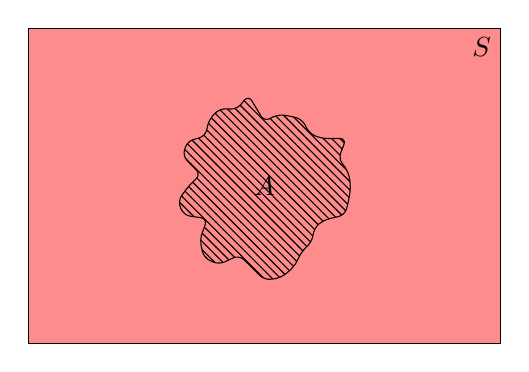
\begin{tikzpicture}
\filldraw[fill=red, fill opacity=.45] (-3,0) rectangle (3,4);
\node[anchor = north east] at (3,4) {$S$};
\coordinate (a) at (0,2);
% \filldraw[fill=yellow, fill opacity = .9, rounded corners=.8mm] (a) \irregularcircle{1cm}{2mm};
\draw[pattern=north west lines, rounded corners=.8mm] (a) \irregularcircle{1cm}{2mm};
\node at (a) {$A$};
\end{tikzpicture}
\caption{Two sets $S$ and $A$ where $S$ contains $A$}
\label{fig:subset}
\end{figure}
How can we describe the relationship between $A$ and $S$ here?  It seems $S$ `contains' $A$ in some sense.  Do we have notation for this?  Well, just like sets have their own definition for `equal to,' they have relations that are (in a \emph{very} loose sense) analogous to `less than or equal to' and `greater than or equal to,' these being the \textbf{subset} and \textbf{superset} relations.\footnote{I have been throwing the word `relation' around a lot without ever defining it.  I `probably' won't define it anywhere in this document, but you might be able to find it in my discrete math notes, assuming I ever TeX them up.}  In a nutshell, these tell us whether one set contains everything that is in the other set:
\begin{sketch}[Subset and Superset Idea]
For two sets $A$ and $B$, $A$ is a \textbf{subset} of $B$ (denoted $A\subseteq B$) if $B$ contains every element of $A$.  Likewise, $A$ is a \textbf{superset} of $B$ (denoted $A\supseteq B$) if $A$ contains every element of $B$. 
\end{sketch}
We actually won't use set-builder notation in our definition here---just like how $\leq$ and $\geq$ are in some sense `related' to = (in that $a=b$ is logically equivalent to saying `$a\leq b$ and $a\geq b$'), saying `$A\subseteq B$ and $A\supseteq B$' is the same as saying $A=B$!  So, we can actually break up our set equality definition into two parts to get our $\subseteq$ and $\supseteq$ definitions:
\begin{leftbar}[.95\linewidth]
\begin{definitiona}[Subset]
For two sets $A$ and $B$, we say $A$ is a \textbf{subset} of $B$ (denoted $A\subseteq B$) if $\forall x\in A$, we also have $x\in B$.  We can also write this as $A\subseteq B$ if $x\in A \Rightarrow x\in B$, which is read as `$A$ is a subset of $B$ if $x$ being in $A$ means that $x$ must also be in $B$.'  If we also have that $A\neq B$, then we say $A$ is a \textbf{proper subset} (or \textbf{strict subset}) of $B$, denoted $A\subset B$.  Note that the difference between $\subseteq$ and $\subset$ is essentially identical to the distinction between $\leq$ and $<$!
\end{definitiona}
\begin{definitiona}[Superset]
For two sets $A$ and $B$, we say $A$ is a \textbf{superset} of $B$ (denoted $A\supseteq B$) if $\forall x\in B$, we also have $x\in A$.  We can also write this as $A\supseteq B$ if $x\in B \Rightarrow x\in A$, which is read as `$A$ is a supersset of $B$ if $x$ being in $B$ means that $x$ must also be in $A$.'  As with subset, if we also have that $A\neq B$, we call $A$ a \textbf{proper superset} (or \textbf{strict superset}) of $B$, denoted $A\supset B$.  
\end{definitiona}
\end{leftbar}
Again, these definitions are very very dense, but they are saying \emph{the same thing} as our sketch.  Not much will be lost if you just think of the definition given in the sketch whenever subsets and supersets come up, but trying to figure out how they're really reflecting the same idea will help you continue becoming more comfortable with mathematical notation.  To this effect, consider why the following examples are true:
\begin{enumerate}
\item In Figure \oldref{fig:subset}, $A\subseteq S$.  
\item $x\in A$ if and only if $\set{x}\subseteq A$\footnote{Scheinerman, \textit{Mathematics: A Discrete Introduction}}
\item $1\not\subseteq\set{-1,0,1}$
\item $\set{1}\subseteq\set{-1,0,1}$
\item $\set{\set{1}}\not\subseteq\set{-1,0,1}$
\item $\varnothing \subseteq \varnothing$ (the empty set is a subset of itself!)
\item For any non-empty set $A$, $\varnothing \subseteq A$ (This is a \textbf{vacuous truth}: because there are no $x\in\varnothing$ to check to see if they're in $A$, then our condition can't fail---i.e., there are no $x\in\varnothing$ that \emph{aren't} in $B$, so we can't say it \emph{isn't} a subset) 
\item For \textbf{any} set $B$, $\varnothing \subseteq B$ 
\item $\set{1}\not\subseteq\set{\set{0,1,2}, \set{1,0}, \set{1}}$
\end{enumerate}
Subsets are
Lastly, consider the red-shaded region in the following diagram:
\begin{figure}[H]
\centering
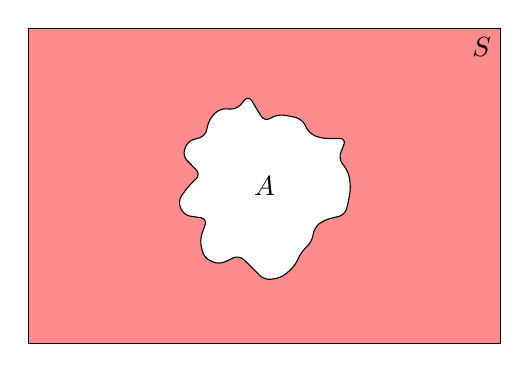
\begin{tikzpicture}
\filldraw[fill=red, fill opacity=.45] (-3,0) rectangle (3,4);
\node[anchor = north east] at (3,4) {$S$};
\coordinate (a) at (0,2);
\filldraw[fill=white, rounded corners=.8mm] (a) \irregularcircle{1cm}{2mm};
\node at (a) {$A$};
\end{tikzpicture}
\caption{The complement of $A$}
\end{figure}
How can we describe this portion?  Well, from the diagram, it looks like $A\subseteq S$, and that the red portion corresponds to $S$ subtracting out all the elements of $A$.  While we won't actually be defining set subtraction here, the idea is similar: we call the red portion of $S$ the \textbf{complement} of $A$ in $S$.  
\begin{sketch}[Set Complement Idea]
Given a set $S$ containing all of $A$, the \textbf{complement} of $A$ in $S$ (denoted $\overline{A}$) is the portion of $S$ that doesn't include anything in $A$.  Note that this means $A\cup \overline{A} = S$! 
\end{sketch}
As has become customary, we must now translate our verbal definition into set-builder notation.  We have been \emph{given} that $A$ is a subset of $S$\footnote{You can think of the phrase `given' as meaning `this definition only applies in the case that (whatever is given) is true.'  Essentially, the phrase `given' tells us what kind of conditions we can assume for our definition/theorem/etc.}, so we're probably going to use this in our definition of the complement.  In particular, we're talking about some \emph{portion} of $S$, so our definition should start with all of $S$, and then apply some other conditions to its elements to get rid of the parts that are also in $A$:
\[\overline{A} = \set{x:x\in S, ????}\]
Where the `????' are other conditions.  We want to make sure that our complement doesn't include any parts of $A$, so we make the next condition $x\notin A$.  This turns out to be our full definition!    
\begin{definition}[Set Complement]
For sets $A$ and $S$ where $A\subseteq S$, the \textbf{complement} of $A$ in the set $S$ (denoted $\overline{A}$) is defined as 
\[\overline{A} = \set{x\in S:x\notin A}\]
\end{definition}
\begin{enumerate}
    \item If $A\subseteq S$, then $A\cap\overline{A} = \varnothing$
    \item If $A\subseteq S$ and $B\subseteq S$, then $\overline{A}\cap\overline{B} = \overline{(A\cup B)}$ (Taken from Rosenlicht.  Break this one down into smaller pieces and apply venn diagrams / set-builder notation.  I'll include a proof later on, but try it on your own first!)
    \item If $A\subseteq S$, then $A = \overline{\overline{A}}$ (the double overline means the complement of the complement!)
\end{enumerate}
%==========================================================================
%
%
%
%
%
%
%
%
%
%
%
%
\subsection{Important Sets of Numbers}
We begin our discussion of important sets of numbers with what most people think of when they hear the word `number.'  A formal definition is pretty unwieldy, so we'll just think of the natural numbers as being \textbf{the positive integers}.  
\begin{definition}[Natural Numbers]
\textbf{Natural numbers} (also called `counting numbers') are positive numbers that can be written without a fractional or decimal component.  Oftentimes, we make statements that involve \textbf{the set of natural numbers}, so we have a special symbol for it: $\NN$.  
\begin{align*}
\NN &= \set{x:x>0, x\text{ can be written without fractions/decimals}} \\ 
&= \set{1,2,3,4,5,\ldots}
\end{align*}
\vspace{-8mm}
\end{definition}
Some texts take the set of natural numbers to include 0 (and interchangably refer to $\NN$ as `whole numbers'), while others don't.  For our purposes, 0 is not a natural number.  But, it's certainly a number of some sort, so $\NN$ on its own doesn't account for \emph{all} numbers---after all, it doesn't contain things like negative numbers and fractions.  We tackle the former first, by cutting the $x>0$ in our definition of the natural numbers.  This gets us the set of $\textbf{integers}$:
\begin{definition}[Integers]
An \textbf{Integer} is any number that can be written without a fraction or decimal.  Just as we have $\NN$ for the set of natural numbers, we also have a special symbol for the set of integers: $\ZZ$ (this comes from the German word for `numbers,' \textit{Zahlen}).  We can think of $\ZZ$ as being the union of the set of natural numbers, the set of their negatives, and $\set{0}$
\[\ZZ = \set{\ldots,-3,-2,-1,0,1,2,3,\ldots}\]
\end{definition}
Still, we don't have a system that adequately addresses things like 1.5, $\frac{3}{7}$, and other numbers.  Now that we have the integers, though, we can construct more numbers:
\begin{definition}[Rational Numbers]
A \textbf{rational number} is any (real) number that can be expressed as the ratio of two integers, provided the denominator is nonzero (we'll talk about the reals later).  We denote \textbf{the set of rational numbers} as $\QQ$ (this was chosen by Giuseppe Peano in 1895, from the italian word for `quotient,' \textit{quoziente}.  As we will see shortly, $\RR$ is already taken...)
\[\QQ = \set{\frac{p}{q}:p,q\in\ZZ, q\neq 0}\]  
In particular, we can express any rational number as a \textbf{simplified} fraction $\frac{p}{q}$.  What `simplified' means is that we can't divide the numerator and denominator by the same thing and get smaller $p$ and $q$.  As an example, a simplified fraction would look something like $\frac{3}{7}$, instead of looking like $\frac{6}{14}$.  In the latter case, we can divide the numerator and denominator by $2$ to get $\frac{3}{7}$, beacuse 6 and 14 share a common factor of 2.  So, if $\frac{p}{q}$ is fully simplified, $p$ and $q$ \textbf{share no common factors} (this is also stated as `$p$ is relatively prime to $q$', and denoted $p\perp q$).
\end{definition}
Note that, for $q=1$, we get the integers back out of $\QQ$, so $\ZZ\subseteq\QQ$.  However, not all numbers can be expressed this way---for instance, $\sqrt{2}$ is not rational (and thus we call it \textbf{irrational}).  The following proof is very similar to that given by \emph{Hippasus}, a 5th century BC mathematician.  The proof, while elegant and short, was not recieved well by his peers---the pythagoreans (a prominent mathematical group at the time, of which he was a member) believed that ``all phenomena in the universe [could] be reduced to whole numbers and their ratios,'' and (by one account) became so enraged upon seeing his proof that they threw him overboard to drown while at sea.\footnote{Quoted a quote from Kline, M. \textit{Mathematical Thought from Ancient to Modern Times}.  I read the quote itself on wikipedia, not in the book.  The page goes on to say that another account holds that Hippasus was `merely' sentenced to exile}  Here is the theorem he showed, and a proof similar to the one he gave:
\begin{theorem}[$\sqrt{2}$ is irrational]
The number $\sqrt{2}$ is irrational; i.e. there exist no $p,q\in\ZZ$ such that $\sqrt{2} = \frac{p}{q}$.
\end{theorem}
In mathematics, when we give a theorem, we (should) always give a proof.  However, direct proof methods are sometimes difficult---in this case, we certainly can't conduct an exhuastive search for different values of $p,q\in\ZZ$ and conclude (after checking them all) that none of them work, because there are \emph{infinite} possible combinations of $p$ and $q$.  Instead, we will use an indirect proof tool: \textbf{proof by contradiction}.
\begin{technique}[Proof by Contradiciton]
\textbf{Proof by contradiction} is an indirect method of proof in which we assume the thing we're proving is false, and show that this assumption leads to some error/contradiction (e.g., that 1=2).  Thus, proposition (the thing we assumed to be false) \emph{cannot} be false, and therefore must be true instead.  This proof method can be especially helpful when direct methods are unfeasible, or when we don't have too much information to base our proof on.  When giving a proof by contradiction, it is common to specify it, so that a reader doesn't get confused by something like `assume all even numbers are odd.'  Typically, we say `suppose, to obtain a contradiction, that...' instead.
\end{technique}
We now prove the statement in question.  The proof is a little tedious, and very indirect (even by the standards of proof by contradiction), so don't worry too much about the details.  The exact mechanics by which we go about obtaining a contraciction \emph{aren't} super important, but do pay attention to the loose structure by which we obtain a contradiction, and how it means our assumption must have been false.  The end of the proof is marked with a $\blacksquare$, which is the modern equivalent of `Q.E.D.'
\begin{leftbar}[.95\linewidth]
\begin{proof}[Proof of Theorem 1.1]
(By contradiction)
Suppose, to obtain a contradiction, that $\sqrt{2}$ is rational.  Then, we can express it as a ratio $\frac{p}{q}$ for some $p,q\in\ZZ$ such that $p$ and $q$ \textbf{share no common factors} (this is true for \emph{any} rational number, so if $\sqrt{2}$ is rational, this must be possible).  So, we have 
\begin{align*}
\sqrt{2} &= \frac{p}{q}, p,q\in\ZZ,q\neq 0, p\perp q
\shortintertext{squaring both sides, we have}
2 &= \frac{p^2}{q^2}
\shortintertext{multiplying both sides by the $q^2$ term yields}
2q^2 &= p^2
\end{align*}
$2q^2$ must be even (because any integer times 2 must be even), so $p^2$ must be even as well, because $p^2$ and $2q^2$ are even.  If a perfect square is even, then its square root must be even as well (odd numbers yield more odd numbers when squared).  Therefore, we have $p$ is even, so $p=2r$ for some integer $r$.  Then, we have 
\begin{align*}
p^2 &= (2r)^2 = 4r^2 
\shortintertext{but $p^2$ also equals $2q^2$, so we can write}
2q^2 &= 4r^2 \\ 
q^2 &= 2r^2
\end{align*}
Since $q^2$ can be written as 2 multiplied by some integer (in this case $r^2$), then $q^2$ is even, and so its square root $q$ must be even as well.  So, we now have that both $p$ and $q$ are even.  But, if $p$ and $q$ are both even, then they share a common factor of 2.  This contradicts our assumption that $p$ and $q$ share no common factors!  Therefore, $\sqrt{2}$ \textbf{cannot} be rational, because all rational numbers can be expressed as a ratio of $p$ and $q$ that don't share common factors.  
\end{proof}
\end{leftbar}
So, we have found one irrational number, $\sqrt{2}$.  By similar proof methods, we can show that the $k^{th}$ root of any integer that is not itself a $k^{th}$ power of an integer is irrational.  Other famously irrational numbers include $\pi$ (the ratio of the circumference of a circle to its diameter), Euler's number $e$ (to be defined later), and the golden ratio $\phi$.  So, we now have a whole handful of irrational numbers!  In fact, it is possible to show that \emph{almost all} real numbers are irrational.\footnote{Here, `almost all' is a technical term that I won't define.  But, to give you some sense of scale, if we were to throw a dart at the real number line, we would actually have a $0\%$ (yes, you read that right) chance of hitting a rational number, because there are infinitely more irrational numbers than rational ones.}  It's strange, then, that there isn't any special symbol to denote the set of all irrational numbers.  This might be because we usually talk about the set of irrational numbers in the context of their union with the set of rational numbers---the \textbf{set of real numbers}.  Unfortunately, I won't give the exact definition of the reals in a more deeply rigorous sense here, as it would escape the scope of our discussion of calculus.  For now, we can think of the reals as being the following:
\begin{definition}[Real numbers]
The \textbf{set of real numbers} is the union of the set of rational numbers ($\QQ$) with the set of irrational numbers.  The \textbf{reals} can also be thought of as the set of all possible distances of points on an infinitely detailed line.  The set of reals is written as $\RR$.
\end{definition}
Thus, we conclude our discussion of important sets of numbers.\footnote{As it turns out, the reals are actually a small subset of the complex field (denoted $\CC$, and consisting of numbers of the form $z=a+bi$, where $i^2 = -1$ and $a,b\in\RR$).  However, in this text we will only deal with the reals, and leave complex functions until another day.}  To summarize what we have discussed in this section with a small picture (not to scale):
\begin{figure}[H]
\centering
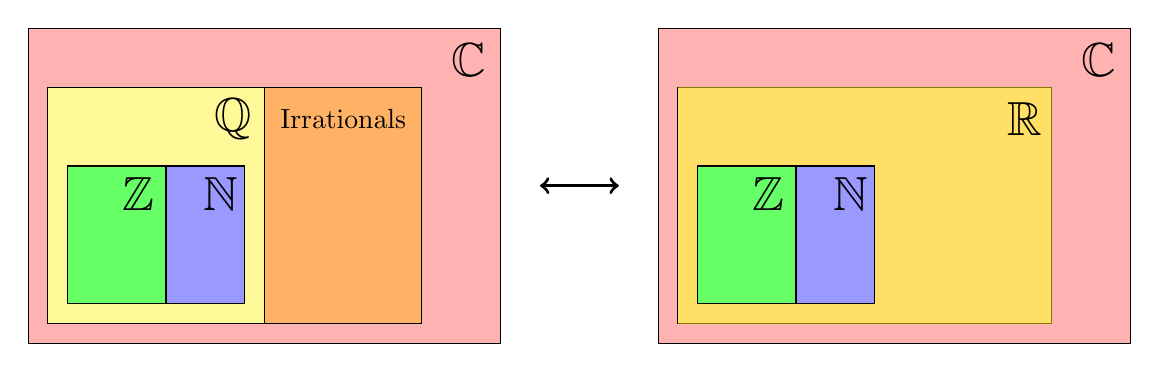
\begin{tikzpicture}
\filldraw[fill=red, fill opacity=.3] (-3,0) rectangle (3,4);
\filldraw[fill=white, fill opacity=1] (-2.75,.25) rectangle (2,3.25);
\filldraw[fill=orange, fill opacity=.6] (0,.25) rectangle (2,3.25);
\filldraw[fill=yellow, fill opacity=.4] (-2.75,.25) rectangle (0,3.25);
\filldraw[fill=white, fill opacity=1] (-2.5,.5) rectangle (-.25,2.25);
\filldraw[fill=green, fill opacity=.6] (-2.5,.5) rectangle (-1.25,2.25);
\filldraw[fill=blue, fill opacity=.4] (-1.25,.5) rectangle (-.25,2.25);
\node (C) at (2.6,3.6) {$\mathop{\mathlarger{\mathlarger{\mathlarger{\mathlarger{\CC}}}}}$};
\node (Q) at (-.4,2.85) {$\mathop{\mathlarger{\mathlarger{\mathlarger{\mathlarger{\QQ}}}}}$};
\node (Z) at (-1.6,1.9) {$\mathop{\mathlarger{\mathlarger{\mathlarger{\mathlarger{\ZZ}}}}}$};
\node (N) at (-.55,1.9) {$\mathop{\mathlarger{\mathlarger{\mathlarger{\mathlarger{\NN}}}}}$};
\node (ir) at (1,2.85) {Irrationals};
%
\draw[<->, very thick] (3.5,2) -- (4.5,2);
%
\filldraw[fill=red, fill opacity=.3] (5,0) rectangle (11,4);
\filldraw[fill=white, fill opacity=1] (5.25,.25) rectangle (10,3.25);
\filldraw[fill=red, fill opacity=.2] (5.25,.25) rectangle (10,3.25);
\fill[fill=yellow, fill opacity=.5] (5.25,.25) rectangle (10,3.25);
\filldraw[fill=white, fill opacity=1] (5.5,.5) rectangle (7.75,2.25);
\filldraw[fill=green, fill opacity=.6] (5.5,.5) rectangle (6.75,2.25);
\filldraw[fill=blue, fill opacity=.4] (6.75,.5) rectangle (7.75,2.25);
\node (C) at (10.6,3.6) {$\mathop{\mathlarger{\mathlarger{\mathlarger{\mathlarger{\CC}}}}}$};
\node (R) at (9.65,2.85) {$\mathop{\mathlarger{\mathlarger{\mathlarger{\mathlarger{\RR}}}}}$};
\node (Z) at (6.4,1.9) {$\mathop{\mathlarger{\mathlarger{\mathlarger{\mathlarger{\ZZ}}}}}$};
\node (N) at (7.45,1.9) {$\mathop{\mathlarger{\mathlarger{\mathlarger{\mathlarger{\NN}}}}}$};
\end{tikzpicture}
\end{figure}
\subsection{Induction}
The techniques we use to solve questions in mathematics can depend heavily on the set we're `dealing with.'  For instance, what call \textbf{calculus} is actually a sub-branch of the larger field of $\textbf{real analysis}$, which is essentially the study of properties of real numbers and their functions.  However, when developing tools we can use to analyze the reals, we will often need to fall back on knowledge of the natural numbers to complete a proof.  So, before proceeding to discussions of functions and their properties, we must first introduce a proof technique that is extremely powerful when dealing with natural numbers: \textbf{induction}.\\~\\
\textbf{Induction} is very useful when we encounter objects with properties that `build on each other' in some way.\footnote{although, it should be noted that this `building' isn't always obvious.  Induction is so powerful though that if you just give it a shot (even if you don't see some kind of obvious iterating pattern), sometimes it'll just work!}  As an example, we might consider the following \textcolor{red}{sum}.  Here, the notation on the left looks fancy, but if we look at the right we can work out that it seems to mean something along the lines of `add the first $n$ natural numbers together.'  %
% Before we continue on to discussion of functions, we'll cover another proof technique.  Oftentimes in mathematics, we seek to prove some property for all natural numbers.  As an example, we might consider the \textcolor{red}{sum} given below.  The notation on the left might look intimidating, but because both sides of the equation must be expressing the same thing, we can use the the right-hand side to understand what the left is asking us.  So, looking at the right, we can see that the greek symbol on the left is telling us `add the first $n$ natural numbers together.'  
\[{\color{red}\sum^{{\color{blue}n}}_{\color{blue} i=0}} ({\color{blue}i}) = \textcolor{blue}{0} \,{\color{red}+}\,\textcolor{blue}{1} \,{\color{red}+}\, \textcolor{blue}{2} \,{\color{red}+}\, \textcolor{blue}{3} \,{\color{red}+}\, \textcolor{blue}{\cdots} \,{\color{red}+}\, \textcolor{blue}{n}\]
Note that here, the $\color{red}\Sigma$ (read as `sigma', which I find helpful to remember by noting `sigma' and `sum' start with the same letter) notation is directly analogous to our $\color{red}\cup$ notation, but here (instead of taking unions), we're taking a \textcolor{red}{sum} of numbers between \textcolor{blue}{0} and $\textcolor{blue}{n}$.  In this sense, just as in the $\color{red}\cup$ notation the big $\color{red}\cup$ on the left hand side of our expression told us we would be taking repeated \textcolor{red}{unions} of sets on the right hand side, here the $\color{red}\Sigma$ on the left hand side informs us we should expect a bunch of \textcolor{red}{addition} (\textcolor{red}{+}) on the right hand side.  While in the $\color{red}\cup$ notation, the big symbol on the left hand side was the same as the little symbols on the right, mathematicians don't use the same convention here.  But, it might be helpful to imagine how the expression would appear if they did:
\[\raisebox{-.45\depth}{$\displaystyle\color{red}\bigplus^{{\color{blue}n}}_{{\color{blue}i=0}}$} ({\color{blue}i}) = \textcolor{blue}{0} \,{\color{red}+}\,\textcolor{blue}{1} \,{\color{red}+}\, \textcolor{blue}{2} \,{\color{red}+}\, \textcolor{blue}{3} \,{\color{red}+}\, \textcolor{blue}{\cdots} \,{\color{red}+}\, \textcolor{blue}{n}\]
Writing out the whole $\textcolor{red}{\Sigma}$ ever time we want to talk about the sum is unwieldy, so we make the following definition:
\[\textcolor{red}{S}(\textcolor{blue}{n}) = {\color{red}\sum^{{\color{blue}n}}_{\color{blue} i=0}} ({\color{blue}i})\]
Occasionally, people use $S(n)$ to denote the actual \emph{number} the \textcolor{red}{sum} returns, and $\Sigma$ to denote the expanded sum itself (i.e, the $1+2+\cdots+n$).  I'll try to stick to this notation.  Now, we can start evaluating the $S(n)$ for the first few values of $n$ to see if we can spot any patterns.
\begin{align*}
S(1) &= 1 \\
S(2) &= 3 \\ 
S(3) &= 6 \\ 
S(4) &= 10 \\ 
S(5) &= 15 \\
&\cvdots
\end{align*}
A formula is not immediately obvious from the numbers given.  But, if we rewrite the right hand side in another way, we can begin to see a pattern taking shape.\footnote{Don't worry for now about \emph{how} we guessed to rewrite the right hand side this way---I'll show how we might have accidentally stumbled upon it in just a little bit.}
\begin{align*}
S(1) &= \frac{1\cdot2}{2} = 1\\ 
S(2) &= \frac{2\cdot3}{2} = 3\\
S(3) &= \frac{3\cdot4}{2} = 6\\ 
S(4) &= \frac{4\cdot5}{2} = 10\\ 
S(5) &= \frac{5\cdot6}{2} = 15\\
&\cvdots
\shortintertext{So, we might conjecture that the sum follows the general formula}
S(n) &= \frac{n\cdot(n+1)}{2}
\end{align*}
However, conjecture is dangerous---there are lots of patterns that hold for small numbers, but turn out to break later on down the line.  In mathematics, if there is even a single value of $n$ (among the infinitely many possible inputs) for which the statement fails, then the statement is said to be \emph{false}.  Not `basically' true, or `almost always correct'---it is false, unless we modify our statement to say `for all $n$ except...'\footnote{After all, the statement `no number is divisible by 15487369' turns out to be true for roughly 99.9994\% of natural numbers.  In many scientific fields, that's basically the same as truth.  But it really misses the point.}  So why don't we just find all the values of $n$ for which it doesn't work, and then specify those in the statement?  Sometimes we can.  Sometimes, there are only a few edge cases we need to consider, othertimes we can exploit patterns in the failures to determine all cases in which the statement will fail.  But, just looking at our equation, it isn't apparent how we could employ any of these strategies.  Instead, we need a consistent tool that we can always use to prove statements of this sort.  To do so, we use the principle of mathematical induction.
\begin{theorem}[The Principle of Mathematical Induction]
Let $S(x)$ be some statement $S$ involving a natural number $x$.  Then, $S(x)$ is true for all natural numbers if 
\begin{enumerate}
    \item The statement holds for $x=1$ \textnormal{(this poriton of the PMI is called `the base case')}.
    \item Whenever $S(k)$ is true, $S(k+1)$ \textbf{must also} be true \textnormal{(this is called `the inductive hypothesis')}.
\end{enumerate}
\end{theorem}
To prove this, we will employ the well-ordering principle, which we introduced in the first secition---it asserts that `every non-empty set of postive integers contains a smallest element.'  Again, the proof here is a little more abstract than the proofs we'll be doing later on, so don't worry about the details, and try to follow generally where the contradiction is happening.  The first few times through, read all of the footnotes in the proof, because they contain logical leaps that I have omitted for the sake of streamlining the proof.  Then, when you feel a little more comfortable with the proof, try reading it straight through a few times, and seeing if the flow of logic makes sense.  If it doesn't try reading with the footnotes again---math, like any language, takes \emph{lots} of practice to get comfortable with.
\begin{leftbar}[.95\linewidth]
\begin{minipage}{\textwidth}
\begin{proof}(By contradiction)
Let's say we have some statement $S(n)$ such that $S(1)$ is true, and furthermore (for $k\in\NN$) whenever $S(k)$ is true, $S(k+1)$ is also true.\footnote{equivalently stated, $S$ is a statement satisfying 1. and 2. of the principle of mathematical induction.}  Suppose, to obtain a contradiciton, that $S(n)$ fails for some natural numbers, and let $A\subseteq\NN$ \textbf{be the set of all natural numbers for which $S$ fails}.  By the well-ordering principle, $A$ must contain a least element.  Let $x$ be this least element.  Then, $S(x)$ must not be true, and so $x$ cannot be 1.\footnote{because we have $S(1)$ is true.}  So, $x\geq 2$.\footnote{because $x$ is a natural number, and one is the smallest natural number, so if $x$ isn't one it must be 2 or larger.}  Then, subtracting a 1 from each side of $x\geq 2$, we have $x-1\geq 1$.\footnote{this is important to show, because if we just had $x-1\geq 0$, then $x-1$ \emph{could} equal 0, and $x-1$ wouldn't necessarily be a natural number, which would mess up the following portion of the proof.}  So $x-1$ is also in $\NN$, and thus, we can apply $S$ to it.  $S(x-1)$ must be true, because $x$ is the \textbf{smallest} natural number for which the statement breaks, so $S$ must be true for any smaller natural number.  But, we know that $S$ is some statement such that if $S(k)$ is true, then $S(k+1)$ must also be true.  So becaues $S(k)$ is true for $k=x-1$, it must also be true for $k+1=x$.\footnote{We have just shown that $S(x)$ must be both true and false!}  This contradicts our assumption that $S(x)$ is false, so such a value of $x$ cannot exist.  This means that, because $x$ was defined as the least element of $A$, $A$ cannot \emph{have} a least element, and so $A$ must be empty!  Thus, the statement fails for no natural numbers.
\end{proof}
\end{minipage}
\end{leftbar}
That proof was very complicated, and its specifics are not \emph{super} important to understanding how induciton works---but, I felt that I should include the proof, even if it is tedious.  In terms of intuition, I like to think of induciton as sort of like building an infinitely long ladder (in this analogy I'll put the corresponding portion of the theorem in parentheses)---the inductive hypothesis says that whenever we're standing on a rung (whenever $S(k)$ is true), we can add another rung above it (we can show that $S(k+1)$ is true).  The base case tells us that we have a starting rung to stand on ($S(1)$ is true).  So, if the base case and inductive hypothesis are both true, then we can build as tall of a ladder as we want (we can show that the statement is true for all natural numbers)!  However, when use induction, we don't \emph{personally} do the metaphorical `construction' of the ladder ourselves (we don't go through and do calculations to show the statement holds for each sequential number): instead, what we show is that it is \emph{possible} to `build the ladder' (i.e., that it is possible to show $S(n)$ for all $n\in\NN$), and the principle of mathematical induction does the actual `building' for us (essentially, the P.M.I says `when it is possible to prove a statement is true for all $n$, it \emph{is true} for all $\NN$') \\~\\
Now that we have shown that the principle of mathematical induction is true, we can begin proving things with it.  The first of the following two examples the is the sum we considered earlier.
\begin{leftbar}[.95\linewidth]
\begin{example}
Let $n\in\NN$.  We seek to prove that the sum of the first $n$ natural numbers is $\frac{n(n+1)}{2}$
\begin{proof}(By induction) First, note that the sum of the first natural number 
\[1 = \frac{1(1+1)}{2} = 1\]
So the statement is true for $n=1$ (the base case).  
Now, suppose the statement is true for $k$, so we have 
\[1+2+\cdots+k = \frac{k(k+1)}{2}\]
Then 
\begin{align*}
1+2+\cdots+k+(k+1) &= \frac{k(k+1)}{2} + (k+1) \\ 
&= \frac{k^2+k}{2} + \frac{2k+2}{2} \\ 
&= \frac{k^2 + 3k + 2}{2} \\ 
&= \frac{(k+1)(k+2)}{2}
\end{align*}
Which exactly the same as $S(k+1)$---so, the statement must hold for $k+1$.  Thus, by the principle of mathematical induction, the statement is true for all natural numbers.
\end{proof}
\end{example}
\end{leftbar}
Even if you managed to follow my poorly-communicated inductive proof, you might be thinking to yourself: \textit{ok, but how was I even supposed to see that pattern in the first place?  The formula given is entirely non-obvious to me when just looking at the numbers $S(n)$ spits out---you must have to be some sort of genius to see things like that.}  I'll let you in on a little secret that I didn't tell you earlier: there is a simpler, geometric way of reasoning about why this identity holds.  In fact, with summation identities like the one we just proved, there often are.  But, geometric ways of reasoning are often more prone to error than inductive proofs are.  In that sense, geometric reasoning is useful in \emph{finding} a pattern, while inductive proof is useful in \emph{proving} the pattern is correct.  \\~\\
Imagine we're back at step 1 of this problem.  We have 
\[S(n) = \sum_{i=0}^n(i) = 1 + 2 + 3 + \cdots + n\]
We want to draw a picture that will help us figure out what's going on.  Specifically, we want a way of relating what's happening in the \emph{expanded sum} (the $1+2+3$ etc) to the actual \emph{number} the sum spits out ($S(n)$).  We're dealing with whole numbers here, so it can be helpful to try drawing out a bunch of identical shapes, like squares or circles (I'll use squares here, and refer to them as `blocks' because I think it's helpful to imagine them stacking on each other).  Let's say each block has an area of 1.  After lots of frustrating trial-and-error, we \emph{might} (it's always a bit of a crapshoot) think of drawing out our blocks in a triangular pile, where each row has 1 more block than the previous row (this corresponds to how the terms in our sum are increasing by 1).  First, we'd start with 1 row of 1 block, writing the total area (which corresponds to $S(n)$) underneath each:
\begin{figure}[H]
\centering
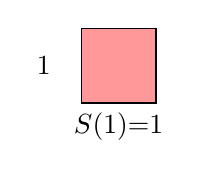
\begin{tikzpicture}[scale=.95]
\foreach \n in {0}{
    \pgfmathsetmacro{\sum}{.5*(\n*(\n+1))};
    \pgfmathsetmacro{\startx}{\sum+2*\n};
    \pgfmathsetmacro{\endx}{\startx+\n};
    \pgfmathsetmacro{\endy}{\n+1};
    \foreach \x in {0,...,\n}{
        \pgfmathsetmacro{\newx}{\x+\startx};
        \foreach \y in {0,1,...,\endy}{
            \pgfmathsetmacro{\labely}{\endy-\y};
            \pgfmathtruncatemacro{\whyyy}{round(\y+1)};
            \ifthenelse{\x=0}
                {\ifthenelse{\y=\endy}
                    {}
                    {\node at (\newx-.5,\labely-.5) {\whyyy}}}
                {}
                ;
            \pgfmathparse{(\x) < 0.001 ? int(1) : int(0)}
            \ifnum\pgfmathresult=1
                \pgfmathparse{(\y) > 1.001 ? int(1) : int(0)}
                \ifnum\pgfmathresult=1
                    \node at (\newx-.5,\y-1) {$+$};
                \fi
            \fi
            \ifthenelse{\y=0}
                {\pgfmathparse{(\x + \y - \n) < 0.001 ? int(1) : int(0)}
                    \ifnum\pgfmathresult=1
                        \fill[fill=red, opacity=.4] (\newx,\y) rectangle (\newx+1,\y+1);
                        \draw (\newx,\y) rectangle (\newx+1,\y+1);
                    \fi}
                {\pgfmathparse{(\x + \y - \n) < 0.001 ? int(1) : int(0)}
                    \ifnum\pgfmathresult=1
                        \fill[fill=green, opacity=.4] (\newx,\y) rectangle (\newx+1,\y+1);
                        \draw (\newx,\y) rectangle (\newx+1,\y+1);
                    \fi}
        }
    }
    \pgfmathsetmacro{\nodex}{.5*(\startx+\endx+1)};
    \pgfmathtruncatemacro{\noden}{round(\n+1)};
    \pgfmathtruncatemacro{\nodesum}{round((\n+1)*(\n+2)*.5)};
    \node[anchor=north] at (\nodex, 0) {$S(\noden)$=\nodesum};
}
\end{tikzpicture}
\end{figure}
Then, we add a second row, so that we have 1 row of 1 block, and 1 row of 2 blocks (here, the new row is shown in red, while the rows we added previously are colored in green):
\begin{figure}[H]
\centering
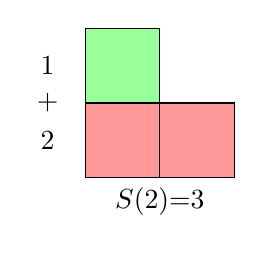
\begin{tikzpicture}[scale=.95]
\foreach \n in {1}{
    \pgfmathsetmacro{\sum}{.5*(\n*(\n+1))};
    \pgfmathsetmacro{\startx}{\sum+2*\n};
    \pgfmathsetmacro{\endx}{\startx+\n};
    \pgfmathsetmacro{\endy}{\n+1};
    \foreach \x in {0,...,\n}{
        \pgfmathsetmacro{\newx}{\x+\startx};
        \foreach \y in {0,1,...,\endy}{
            \pgfmathsetmacro{\labely}{\endy-\y};
            \pgfmathtruncatemacro{\whyyy}{round(\y+1)};
            \ifthenelse{\x=0}
                {\ifthenelse{\y=\endy}
                    {}
                    {\node at (\newx-.5,\labely-.5) {\whyyy}}}
                {}
                ;
            \pgfmathparse{(\x) < 0.001 ? int(1) : int(0)}
            \ifnum\pgfmathresult=1
                \pgfmathparse{(\y) > 1.001 ? int(1) : int(0)}
                \ifnum\pgfmathresult=1
                    \node at (\newx-.5,\y-1) {$+$};
                \fi
            \fi
            \ifthenelse{\y=0}
                {\pgfmathparse{(\x + \y - \n) < 0.001 ? int(1) : int(0)}
                    \ifnum\pgfmathresult=1
                        \fill[fill=red, opacity=.4] (\newx,\y) rectangle (\newx+1,\y+1);
                        \draw (\newx,\y) rectangle (\newx+1,\y+1);
                    \fi}
                {\pgfmathparse{(\x + \y - \n) < 0.001 ? int(1) : int(0)}
                    \ifnum\pgfmathresult=1
                        \fill[fill=green, opacity=.4] (\newx,\y) rectangle (\newx+1,\y+1);
                        \draw (\newx,\y) rectangle (\newx+1,\y+1);
                    \fi}
        }
    }
    \pgfmathsetmacro{\nodex}{.5*(\startx+\endx+1)};
    \pgfmathtruncatemacro{\noden}{round(\n+1)};
    \pgfmathtruncatemacro{\nodesum}{round((\n+1)*(\n+2)*.5)};
    \node[anchor=north] at (\nodex, 0) {$S(\noden)$=\nodesum};
}
\end{tikzpicture}
\end{figure}
We continue adding a new bottom row in this fashion:
\begin{figure}[H]
\centering
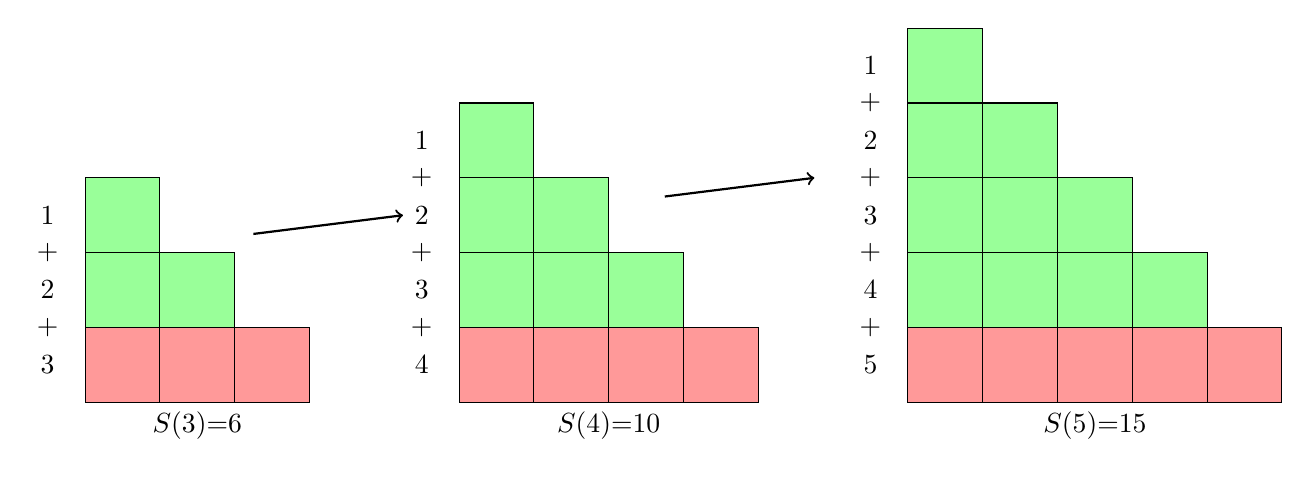
\begin{tikzpicture}[scale=.95]
\foreach \n in {2,3,4}{
    \pgfmathsetmacro{\sum}{.5*(\n*(\n+1))};
    \pgfmathsetmacro{\startx}{\sum+2*\n};
    \pgfmathsetmacro{\endx}{\startx+\n};
    \pgfmathsetmacro{\endy}{\n+1};
    \foreach \x in {0,...,\n}{
        \pgfmathsetmacro{\newx}{\x+\startx};
        \foreach \y in {0,1,...,\endy}{
            \pgfmathsetmacro{\labely}{\endy-\y};
            \pgfmathtruncatemacro{\whyyy}{round(\y+1)};
            \ifthenelse{\x=0}
                {\ifthenelse{\y=\endy}
                    {}
                    {\node at (\newx-.5,\labely-.5) {\whyyy}}}
                {}
                ;
            \pgfmathparse{(\x) < 0.001 ? int(1) : int(0)}
            \ifnum\pgfmathresult=1
                \pgfmathparse{(\y) > 1.001 ? int(1) : int(0)}
                \ifnum\pgfmathresult=1
                    \node at (\newx-.5,\y-1) {$+$};
                \fi
            \fi
            \ifthenelse{\y=0}
                {\pgfmathparse{(\x + \y - \n) < 0.001 ? int(1) : int(0)}
                    \ifnum\pgfmathresult=1
                        \fill[fill=red, opacity=.4] (\newx,\y) rectangle (\newx+1,\y+1);
                        \draw (\newx,\y) rectangle (\newx+1,\y+1);
                    \fi}
                {\pgfmathparse{(\x + \y - \n) < 0.001 ? int(1) : int(0)}
                    \ifnum\pgfmathresult=1
                        \fill[fill=green, opacity=.4] (\newx,\y) rectangle (\newx+1,\y+1);
                        \draw (\newx,\y) rectangle (\newx+1,\y+1);
                    \fi}
        }
    }
    \pgfmathsetmacro{\nodex}{.5*(\startx+\endx+1)};
    \pgfmathtruncatemacro{\noden}{round(\n+1)};
    \pgfmathtruncatemacro{\nodesum}{round((\n+1)*(\n+2)*.5)};
    \node[anchor=north] at (\nodex, 0) {$S(\noden)$=\nodesum};
    \pgfmathsetmacro{\arrow}{\n*.5+1.25};
    \pgfmathsetmacro{\arrowb}{\startx+\arrow};
    \pgfmathsetmacro{\arrowa}{\arrow+(\n*5-1)};
    \ifthenelse{\n=4}
    {}
    {\draw[->,thick] (\arrowb,\arrow) -- (\arrowa,\arrow+.25)}
    ;
}
\end{tikzpicture}
\end{figure}
It seems to hold nicely, so let's see if we can find a way to relate the sum (shown on the left-hand side of the triangle) to the area ($S(n)$) using geometry.  We have a bunch of nice rectangular blocks, so maybe we should try to think about how we could find a way of relating the total area of our piles to the area of a big rectangle.  Looking at our piles, we might think `hmm, that looks kinda like a square but with a bite taken out of it (here, the pile is in red, and the `bite' in white):'
\begin{figure}[H]
\centering
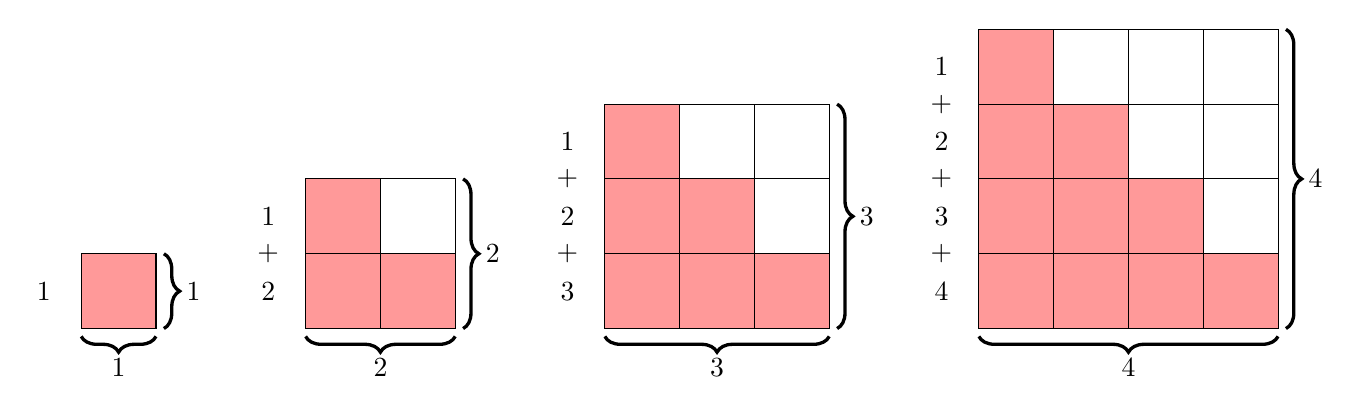
\begin{tikzpicture}[scale=.95]
\foreach \n in {0,1,2,3}{
    \pgfmathsetmacro{\sum}{.5*(\n*(\n+1))};
    \pgfmathsetmacro{\startx}{\sum+2*\n};
    \pgfmathsetmacro{\endx}{\startx+\n};
    \pgfmathsetmacro{\endy}{\n};
    \foreach \x in {0,...,\n}{
        \pgfmathsetmacro{\newx}{\x+\startx};
        \foreach \y in {0,...,\endy}{
            \pgfmathsetmacro{\labely}{\endy-\y};
            \pgfmathtruncatemacro{\whyyy}{round(\y+1)};
            \ifthenelse{\x=0}
                {\node at (\newx-.5,\labely+.5) {\whyyy}}
                {}
                ;
            \pgfmathparse{(\x) < 0.001 ? int(1) : int(0)}
            \ifnum\pgfmathresult=1
                \pgfmathparse{(\y) > 0.001 ? int(1) : int(0)}
                \ifnum\pgfmathresult=1
                    \node at (\newx-.5,\y) {$+$};
                \fi
            \fi
            \pgfmathparse{(\x + \y - \n) < 0.001 ? int(1) : int(0)}
            \ifnum\pgfmathresult=1
                \fill[fill=red, opacity=.4] (\newx,\y) rectangle (\newx+1,\y+1);
            \fi
            \draw (\newx,\y) rectangle (\newx+1,\y+1);
        }
    }
    \pgfmathtruncatemacro{\bracen}{round(\n+1)};
    \pgfmathtruncatemacro{\bracena}{round(\n+1)};
    \draw[very thick, decoration={brace, raise=.1cm, amplitude=.2cm, mirror}, decorate] (\startx, 0) -- (\endx+1, 0) node[pos=.5,anchor=north,yshift=-.25cm] {\bracen};
    \draw[very thick, decoration={brace, raise=.1cm, amplitude=.2cm, mirror}, decorate] (\endx+1, 0) -- (\endx+1, \endy+1) node[pos=.5,anchor=west,xshift=.25cm] {\bracena};
}
\end{tikzpicture}
\end{figure}
So then our area would be $n^2-\text{area of bite}$.  However, we're actually back to where we started now---each of the `bites' is just the area of the red section to the left.  So, expressed as an equation:
\[S(n) = n^2 - S(n-1)\]
Which doesn't seem solvable.\footnote{Actually, it \emph{is} solvable.  It's called a \textbf{recurrence relation}, and I might write about them in my Discrete Math notes.  But, we won't talk about recurrence relations here.}  If we only had a $S(n)$ instead of a $S(n-1)$ on the other side, then we could actually solve the equation, because we could say 
\begin{align*}
S(n) &= n^2 - S(n) 
\shortintertext{in which case adding $S(n)$ to both sides cancels the $S(n)$ on the right, yielding}
2S(n) &= n^2 \\ 
S(n) &= \frac{n^2}{2}
\end{align*}
Which would make our lives much easier.  But wait---what if we added another row to the `bite,' so that we \emph{could} make some statement of the sort?
\begin{figure}[H]
\centering
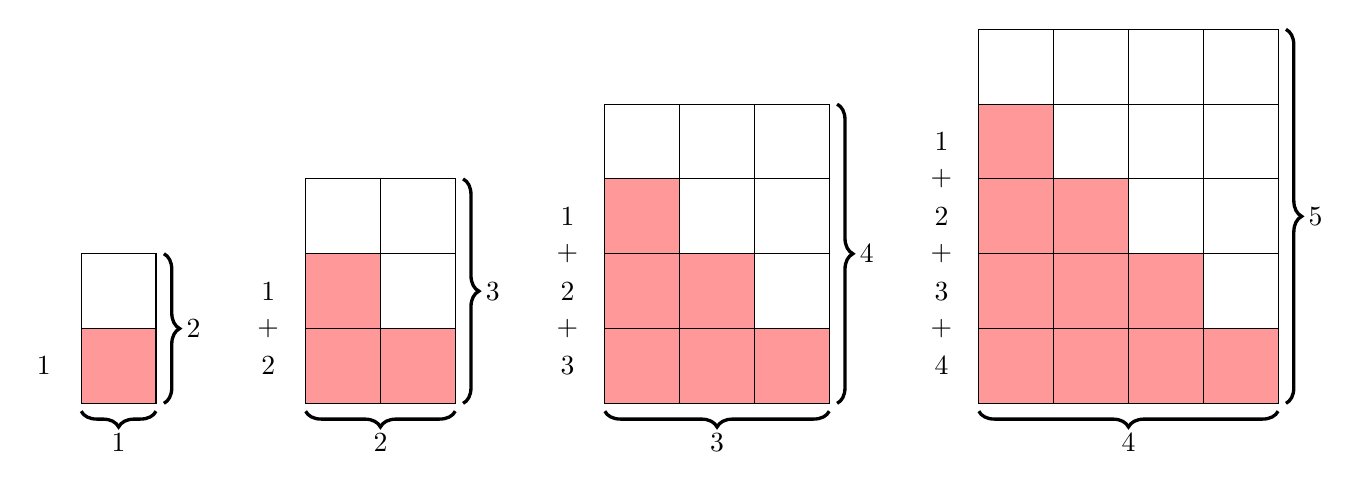
\begin{tikzpicture}[scale=.95]
\foreach \n in {0,1,2,3}{
    \pgfmathsetmacro{\sum}{.5*(\n*(\n+1))};
    \pgfmathsetmacro{\startx}{\sum+2*\n};
    \pgfmathsetmacro{\endx}{\startx+\n};
    \pgfmathsetmacro{\endy}{\n+1};
    \foreach \x in {0,...,\n}{
        \pgfmathsetmacro{\newx}{\x+\startx};
        \foreach \y in {0,1,...,\endy}{
            \pgfmathsetmacro{\labely}{\endy-\y};
            \pgfmathtruncatemacro{\whyyy}{round(\y+1)};
            \ifthenelse{\x=0}
                {\ifthenelse{\y=\endy}
                    {}
                    {\node at (\newx-.5,\labely-.5) {\whyyy}}}
                {}
                ;
            \pgfmathparse{(\x) < 0.001 ? int(1) : int(0)}
            \ifnum\pgfmathresult=1
                \pgfmathparse{(\y) > 1.001 ? int(1) : int(0)}
                \ifnum\pgfmathresult=1
                    \node at (\newx-.5,\y-1) {$+$};
                \fi
            \fi
            \pgfmathparse{(\x + \y - \n) < 0.001 ? int(1) : int(0)}
            \ifnum\pgfmathresult=1
                \fill[fill=red, opacity=.4] (\newx,\y) rectangle (\newx+1,\y+1);
            \fi
            \draw (\newx,\y) rectangle (\newx+1,\y+1);
        }
    }
    \pgfmathtruncatemacro{\bracen}{round(\n+1)};
    \pgfmathtruncatemacro{\bracena}{round(\n+2)};
    \draw[very thick, decoration={brace, raise=.1cm, amplitude=.2cm, mirror}, decorate] (\startx, 0) -- (\endx+1, 0) node[pos=.5,anchor=north,yshift=-.25cm] {\bracen};
    \draw[very thick, decoration={brace, raise=.1cm, amplitude=.2cm, mirror}, decorate] (\endx+1, 0) -- (\endx+1, \endy+1) node[pos=.5,anchor=west,xshift=.25cm] {\bracena};
}
\end{tikzpicture}
\end{figure}
Because of this extra row we've added, we no longer have a perfect square---now, we have a bunch of rectangles that appear to have width $n$ and height $n+1$.  The formula for area of a rectangle is $A=w\cdot h$ (where $w$ is width, $h$ is height, and $A$ is area), so we can say $A=n\cdot(n+1)$.  Now, we have 
\begin{align*}
S(n) &= A - S(n) \\
2S(n) &= A
\shortintertext{Substituting for $A=n(n+1)$,}
2S(n) &= n\cdot(n+1)\\ 
S(n) &= \boxed{\frac{n\cdot(n+1)}{2}}
\end{align*}
Now, we have a pattern, and we can verify it with induction!  Right about now, you might be questioning why we even \emph{need} induction---our geometric reasoning was (in my opinion at least) \emph{much} easier to follow than the inductive proof, so why not just use geometric proofs all the time?  When can that fail?  Well, consider the number of regions that $n$ random points on the rim of a circle divide it into:
\begin{figure}[H]
    \centering
    \begin{minipage}{.3\textwidth}
        \begin{tikzpicture}
            \draw (0,0) circle (2cm);
        \end{tikzpicture}
    \end{minipage}
        \begin{minipage}{.3\textwidth}
            \begin{tikzpicture}
                \draw (0,0) circle (2cm);
                \node[circle,draw=black,fill=white] (0) at (1.9577727873003192,-0.40881011888936736){};
            \end{tikzpicture}
        \end{minipage}
    \begin{minipage}{.3\textwidth}
        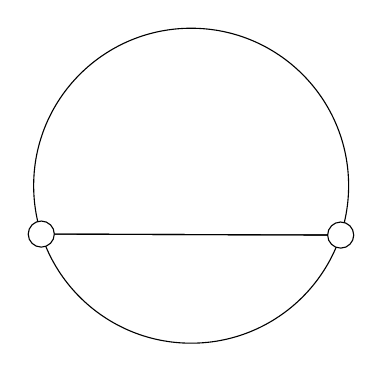
\begin{tikzpicture}
            \draw (0,0) circle (2cm);
            \node[circle,draw=black,fill=white] (0) at (1.899215666417394,-0.626881051264699){};
            \node[circle,draw=black,fill=white] (1) at (-1.9033228844288725,-0.6142979713537696){};
            \draw (0) -- (1);
            \draw (1) -- (0);
        \end{tikzpicture}
    \end{minipage}
\end{figure}
%
%
%
%
\begin{figure}[H]
    \centering
    \begin{minipage}{.3\textwidth}
        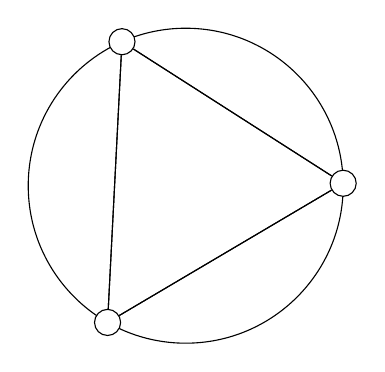
\begin{tikzpicture}
        \draw (0,0) circle (2cm);
        \node[circle,draw=black,fill=white] (0) at (1.9997603173110738,0.030962449966265047){};
        \node[circle,draw=black,fill=white] (1) at (-0.8094818400201633,1.8288628025845926){};
        \node[circle,draw=black,fill=white] (2) at (-0.9924331253337969,-1.7363975615452218){};
        \draw (0) -- (1);
        \draw (0) -- (2);
        \draw (1) -- (0);
        \draw (1) -- (2);
        \draw (2) -- (0);
        \draw (2) -- (1);
        \end{tikzpicture}
    \end{minipage}
%
    \begin{minipage}{.3\textwidth}
        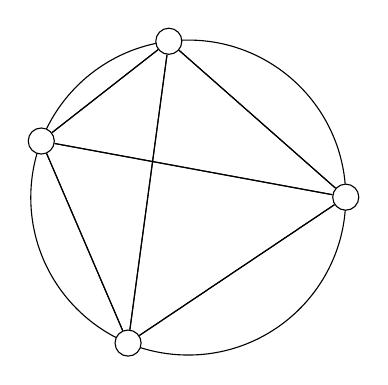
\begin{tikzpicture}
        \draw (0,0) circle (2cm);
        \node[circle,draw=black,fill=white] (0) at (1.9999939602810288,0.004915164229845774){};
        \node[circle,draw=black,fill=white] (1) at (-0.24696314839019326,1.9846937303617411){};
        \node[circle,draw=black,fill=white] (2) at (-1.8667458424078835,0.7178161044814202){};
        \node[circle,draw=black,fill=white] (3) at (-0.7643384938599779,-1.8481846949923215){};
        \draw (0) -- (1);
        \draw (0) -- (2);
        \draw (0) -- (3);
        \draw (1) -- (0);
        \draw (1) -- (2);
        \draw (1) -- (3);
        \draw (2) -- (0);
        \draw (2) -- (1);
        \draw (2) -- (3);
        \draw (3) -- (0);
        \draw (3) -- (1);
        \draw (3) -- (2);
        \end{tikzpicture}
    \end{minipage}
    \begin{minipage}{.3\textwidth}
        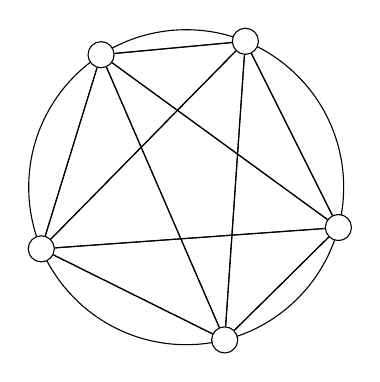
\begin{tikzpicture}
        \draw (0,0) circle (2cm);
        \node[circle,draw=black,fill=white] (0) at (1.933349816594461,-0.5120141469472932){};
        \node[circle,draw=black,fill=white] (1) at (0.7517324721409848,1.8533478600437652){};
        \node[circle,draw=black,fill=white] (2) at (-1.0810264808913184,1.6826710158589324){};
        \node[circle,draw=black,fill=white] (3) at (-1.8404173246874014,-0.7828563539950788){};
        \node[circle,draw=black,fill=white] (4) at (0.4888756636122012,-1.9393299320970967){};
        \draw (0) -- (1);
        \draw (0) -- (2);
        \draw (0) -- (3);
        \draw (0) -- (4);
        \draw (1) -- (0);
        \draw (1) -- (2);
        \draw (1) -- (3);
        \draw (1) -- (4);
        \draw (2) -- (0);
        \draw (2) -- (1);
        \draw (2) -- (3);
        \draw (2) -- (4);
        \draw (3) -- (0);
        \draw (3) -- (1);
        \draw (3) -- (2);
        \draw (3) -- (4);
        \draw (4) -- (0);
        \draw (4) -- (1);
        \draw (4) -- (2);
        \draw (4) -- (3);
        \end{tikzpicture}
    \end{minipage}
\end{figure}
A fantastic youtube channel, 3Blue1Brown, poses the following puzzle in one of his videos (\url{https://youtu.be/84hEmGHw3J8}):
\begin{leftbar}[.95\linewidth]
\begin{minipage}{.3\textwidth}
    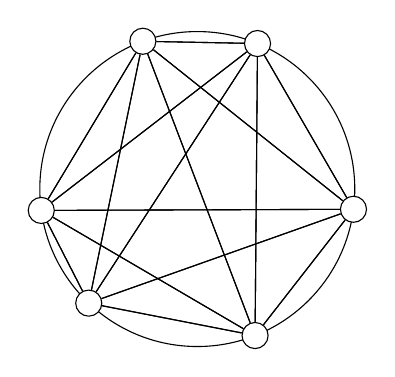
\begin{tikzpicture}
        \draw (0,0) circle (2cm);
        \node[circle,draw=black,fill=white] (0) at (1.9834114866469035,-0.25705811529130995){};
        \node[circle,draw=black,fill=white] (1) at (0.7650728334997134,1.847880829339576){};
        \node[circle,draw=black,fill=white] (2) at (-0.6915086046668064,1.87665016709875){};
        \node[circle,draw=black,fill=white] (3) at (-1.9814539230756594,-0.2717358105367765){};
        \node[circle,draw=black,fill=white] (4) at (-1.3786354842417663,-1.4489182867192583){};
        \node[circle,draw=black,fill=white] (5) at (0.7338580009672189,-1.8604978996001036){};
        \draw (0) -- (1);
        \draw (0) -- (2);
        \draw (0) -- (3);
        \draw (0) -- (4);
        \draw (0) -- (5);
        \draw (1) -- (0);
        \draw (1) -- (2);
        \draw (1) -- (3);
        \draw (1) -- (4);
        \draw (1) -- (5);
        \draw (2) -- (0);
        \draw (2) -- (1);
        \draw (2) -- (3);
        \draw (2) -- (4);
        \draw (2) -- (5);
        \draw (3) -- (0);
        \draw (3) -- (1);
        \draw (3) -- (2);
        \draw (3) -- (4);
        \draw (3) -- (5);
        \draw (4) -- (0);
        \draw (4) -- (1);
        \draw (4) -- (2);
        \draw (4) -- (3);
        \draw (4) -- (5);
        \draw (5) -- (0);
        \draw (5) -- (1);
        \draw (5) -- (2);
        \draw (5) -- (3);
        \draw (5) -- (4);
    \end{tikzpicture}
\end{minipage}
\begin{minipage}{.69\textwidth}
Take two points on a circle, and draw a line straight through. \\
The space which was encircled is divided into two. \\
To these points add a third one, which gives us two more chords: \\
The space through which these lines run has been fissured into four. \\
Continue with the fourth point, and three more lines drawn straight, \\
Now the count of disjoint regions sums, in all, to eight. \\
A fifth point and its four lines support this pattern gleaned, \\
Counting sections one divines that there are now sixteen. \\
This pattern here of doubling does seem a sturdy one, \\
But one more step is troubling as the sixth gives thirty-one.
\end{minipage}
\end{leftbar}
Go ahead, count them!  At first glance, the rule of doubling seems very reasonable.  Loosely speaking, every time we add a point to the rim, we're cutting a bunch of the preexisting regions in two, leaving some intact, and cutting some others multiple times.  For the first few iterations, the regions we cut multiple times `balance out' the regions we only cut once, so it'd be easy to think `every time we add a point to the rim, we double the number of regions.'  Geometrically, it's not incredibly intuitive, but it does seem plausible.  And checking the first few iterations, the pattern would hold so well that we might accept it without questioning it---but if you were to try and prove this inductively, you'd fail, because it's false.
\begin{leftbar}[.95\linewidth]
Try to find patterns (geometrically or otherwise) in the following exercises, and prove them inductively:
\begin{enumerate}
    \item The sum of the first $n$ odd numbers (note that the $n^{th}$ odd number is $2n-1$) \[S(n) = \sum_{i=0}^n(2n-1) = 1 + 3 + 5 + \cdots + (2n-1)\]
    \item The sum of the first $n$ powers of 2 \[S(n) = \sum_{i=0}^n(2^i) = 2^0 + 2^1 + 2^2 + \cdots + 2^n\]
\end{enumerate}
\end{leftbar}
I'll give the inductive proof for the first, but won't include diagrams.  For the geometric part, grab some graph paper and shade in some squares in a similar manner to what we did with the diagrams for the previous example---make sure you're making each $S(n)$ out of a rectangle!
\begin{leftbar}[.95\linewidth]
\begin{example}
Let $n\in\NN$.  We seek to prove that the sum of the first $n$ odd numbers is $n^2$
\begin{proof}(By induction) First, note that the sum of the odd number
\[1 = 1^2 = 1\]
So the statement is true for $n=1$ (the base case).  
Now, suppose the statement is true for $k$.  The $k^{th}$ natural number is $2k-1$, so we have 
\[1+3+\cdots+(2k-1) = k^2\]
Then 
\begin{align*}
1+3+\cdots+(2k-1)+(2(k+1)-1) &= 1+3+\cdots+(2k-1)+(2k+2-1) \\ 
&= k^2 + (2k+1) \\ 
&= (k+1)^2
\end{align*}
Which exactly the same as $S(k+1)$!  So, the statement must hold for $k+1$.  Thus, by the principle of mathematical induction, the statement is true for all natural numbers.
\end{proof}
\end{example}
\end{leftbar}
\begin{leftbar}[.95\linewidth]
Some more exercises, this time with things other than sums (don't be intimidated---the core reasoning is identical!)
\begin{enumerate}
    \item Prove (inductively) that \[\sum_{i=0}^n (10^i) < 10^{n+1}\] holds for all $n\in\NN$
    \item Prove that $4^n-1$ is divisible by 3
    \item Here's a non-example (that is, a pattern that appears to hold, but actually fails later down the line): Show that the following statement is false:
    \[\forall n\in\NN, n^2+n+41 \text{ is prime.}\]
    Note that a \textbf{prime} is defined as a natural number greater than 1 that has no positive divisors other than 1 and itself.  You will want to solve this problem by finding a \textbf{counterexample}---i.e., a value of $n$ for which the statement is false.  \textbf{DO NOT} brute force this problem!  Initially, a solution \textbf{will not} be obvious---but don't be discouraged!  If you find yourself spending more than 10-15 minutes on the solution, \textbf{put it down} and come back to it whenever you feel like it.  There is a non-obvious logical leap required here---try to think about how you can exploit the definition of a prime number in a relatively `simple' way!
\end{enumerate}
\end{leftbar}
\clearpage
\section{Functions of Real Numbers}
\subsection{Functions}
\subsubsection{What is a Function?}
So, what really \emph{is} a function?  Oftentimes, functions are usually taught to students in one of a few ways:
\begin{enumerate}
    \item A function is an \textbf{formula}, e.g. $f(x) = x^2$
    \item A function is a `black box' that you plug a number into.  The function then spits out another number.  E.g., if we plug 2 into $f(x) = x^2$, we get $f(2) = 2^2 = 4$.
\end{enumerate}
Really, these aren't bad ways of describing what's actually happening (most of the time).  But, both are descriptions of what functions can do and/or look like, not what functions fundamentally \emph{are}, because they conflate the function (this is $f$) with what it outputs for some value of $x$ (this is $f(x)$).  And if we poke at these definitions for long enough, they begin to feel less than satisfactory---in particular, they make functions sound like some kind of mechanical process wherein you plug some number $x$ into a function, the function applies a bunch of wacky transformations to your particular $x$, and then spits the finished product back out to you.  For polynomials, this process makes some sense; to some extent it's possible to `wrap your head' around what is happening when you plug $2$ into $f(x)=x^2$.  But when we deal with things like $f(x) = \sin(x)$, this definition becomes a lot sketchier.  I mean, what exactly \emph{are} the transformations going on with $\sin(x)$?  If we ask Wolfram Alpha what $\sin(2)$ is, it spits out
\[\sin(2) = 0.90929742682568169539601986591174484270225497144789026837897301153096730154078354462...\]
Seriously, what kind of black magic does $\sin(x)$ have to be pulling to turn a number as `ordinary' and `nice' as \emph{2} into that garbage?  It turns out that, not only is $\sin(2)$ irrational (and thus, its decimal representation is infinite and contains no repeating `pattern' in its digits), it's actually an even \emph{more} confounding type of number---a \textbf{trancendental number} (more on these much later).  We can trick ourselves into thinking we're gaining insight by examining what's called a \textbf{Taylor Series}---what this means is, as we will see later, we can actually express $\sin(x)$ as the infinite polynomial 
\[\sin(x) = \sum_{i=0}^\infty\left(\frac{(-1)^n\cdot x^{2n+1}}{(2n+1)!}\right) = \frac{x}{1!} - \frac{x^3}{3!} + \frac{x^5}{5!} - \frac{x^7}{7!} + \cdots + \frac{(-1)^n\cdot x^{2n+1}}{(2n+1)!} + \cdots \]
But I mean come on---that's almost just as unhelpful as if we hadn't said anything in the first place.  Because we're adding an \emph{infinite} number of terms together here, even if we were to spend billions of years crunching out inreasingly-precise values for $\sin(2)$, we'd still never get \emph{any} closer to finding out what its value \emph{actually is}.  Yet $\sin(2)$ certainly has \emph{some} value that definitely exists.  For, it can be defined as the height of a point $2$ radians ($\approx$114.592\textdegree, shown in red in the diagram) of the way along a circle of radius 1:
\begin{figure}[H]
\centering
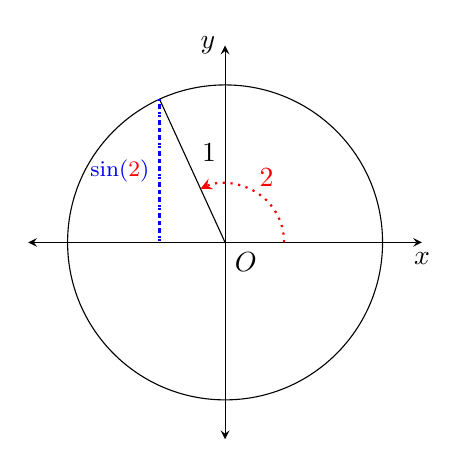
\begin{tikzpicture}[>=latex]
  \tikzset{>=stealth}
  % draw axes and labels. We store a single coordinate to have the
  % direction of the x axis
  \draw[<->] (-2.5,0) -- ++(5,0) coordinate (X) node[below] {$x$};
  \draw[<->] (0,-2.5) -- ++(0,5) node[left] {$y$};

  \newcommand\CircleRadius{2cm}
  \draw (0,0) circle (\CircleRadius);
  % special method of noting the position of a point
  \coordinate (P) at (114.592:\CircleRadius);

  \draw 
  (0,0) 
  coordinate (O) % store origin
  node[below right] {$O$} % label
  -- 
  node[above left,pos=1] {}%{$P(x,y)$} % some labels
  node[above right,midway] {$1$}
  (P);
  \draw[thick,dotted, blue] (P)
  -- 
  node[midway,left] {\footnotesize$\sin(\textcolor{red}{2})$}
  (P |- O) coordinate (Px) % projection onto horitontal line through
                           % O, saved for later
  -- 
  node[midway,below] {}%{$\cos(\textcolor{red}{2})$}
  cycle % closed path
  % pic trick is from the angles library, requires the three points of
  % the marked angle to be named
  pic [draw,red,->,angle radius=.75cm,pic text=$2$,
  angle eccentricity=1.3] {angle=X--O--P};

  % right angle marker
  % \draw ($(Px)+(0.3,0)$) -- ++(0,0.3) -- ++(-0.3,0);
\end{tikzpicture}
\caption{The unit circle}
\end{figure}
So, functions certainly must have \emph{values} at their inputs (provided the function is \textbf{defined} there, a term we'll cover later), regardless of whether or not we can actually compute a decimal representation of these values.  So, we can very loosely describe a function as `something that has values for different inputs.'  However, there is one caveat: our function must give \emph{the same output} for a given input every time.\footnote{Note that this just part of what mathematicians defined the word `function' to mean; we haven't derived this fact anywhere.}  I.e., if we had 
\[f(2) = 4 \text{ and } f(3) = 4\]
That would be fine---having the same output for more than one input is ok. If, on the other hand, we had something like
\[g(2) = 4 \text{ and } g(2) = 3\]
then $g$ cannot be a function, because it gives us two different values when we plug in $2$.  Let's try to incorporate that into a definition:
\begin{sketch}[Function Idea I]
A \textbf{function} is something that associates each input with exactly one output (also called the \textbf{image}).  In this sense, what makes something a `function' is that it is \emph{consistent}---e.g., if we have a function $f$, then when we plug 2 into $f(x)$, we should get the same output every single time.  However, it's perfectly acceptable for one output to be associated with more than one input, because functions only `go in one direction' (input $\rightarrow$ output).
\end{sketch}
This is a pretty good definition for a function---and to be honest, not much will be lost to the reader who just thinks of the above sketch as the definition of a function.  In fact, during most of our exploration of calculus, it'll probably be the best way to think about the material we're discussing (at least, on an intuitive level).  But, it is good to have a more formal understanding of what functions are so that you can refer back to it whenever a more involved proof requires the definition.  With that in mind, let's probe at some of the weakenesses of our sketch.  The main issue I see is in our use of the word `associates'---what does that mean?  What do these associations look like?  How are they stored, and what formal objects that we've already introduced can we use to talk about them?  Well, seeing as they're all I've introduced in this text so far, it's probably pretty safe to say we're probably going to be using sets or lists in some manner.  One possible way is to record every possible input ($x$), and put it in an ordered pair with some output ($f(x)$) (note that how we assign the outputs \emph{does not affect} $f$'s status as a function---if we choose our outputs randomly, it might not be a particularly \emph{interesting} or \emph{clean} function, but it'd still be a function).  In other words, we'd be making ordered pairs like these
\[(\text{input},\text{output}) = (x,f(x))\]
For every possible input $x$, and its corresponding output $f(x)$.    While not particularly elegant, this actually gets the job done pretty well!  Then, we could define our function as the \emph{set} of all these input-output pairs:
\[f = \set{(x,f(x)):x\text{ is an input, and $f(x)$ is an output we've assigned it}}\]
Note here that, although I talk about `assigning' outputs, usually \emph{we won't be going through and assigning these ourselves}.  This is describing how we \emph{could} go about constructing a function, but for the majority of the text here, the functions we'll be dealing with will be abstract mathematical objects that \emph{have already been constructed} (this distinction will make more sense later).  Anyways, we can use the set-builder notation above as an idea for how to more formally define a function:
\begin{sketch}[Function Idea II]
A \textbf{function} (also called a \textbf{mapping} or \textbf{map}, typically denoted with lower-case letters) is a set of ordered pairs of inputs and outputs.  If our function is named $f$, then these ordered pairs would look like $(x,f(x))$.  How these pairs are determined isn't actually important; what matters is only that each input is associated with \emph{only} one output.
\end{sketch}
So, as an example, 
\[f = \set{(2,3),(3,4)}\]
is a function, but 
\[g = \set{(2,4),(2,3)}\]
is not, because $f(2)$ could equal 4 \emph{or} 3.\footnote{We can't just pick one of the two values to be what $f(2)$ `really' means, because any tie-breaking method seems arbitrary.  Should we pick the larger value?  The one that is most similar to other outputs?  Whichever one is closer to the input?  This kind of ambiguity would make it impossible to talk about lots of the cool properties functions have, so define functions to be sets in which each $x$ is paired with one (and only one) $f(x)$.  This might seem a little arbitrary to you---but, we aren't just pretending the troublesome sets don't exist.  Instead, we're \emph{limiting the scope of our discussion}, because it turns out that the objects we've just described as `functions' have some really cool properties.}  Note that functions \emph{don't have to work for all values of $x$ that we can think of}!  For instance, if we look at the $f$ we defined above, if we asked what $f(1)$ was, we wouldn't know what to do---$f$ doesn't tell us anything about how it treats 1.  In this case, we say $f(1)$ is \textbf{undefined}, which essentially means that asking for $f(1)$ is nonsensical.  This brings us to three pieces of vocabulary that are extremely useful when talking about functions: \textbf{domain}, \textbf{image}, and \textbf{codomain}.  Here, we give a definition of \textbf{domain} and \textbf{image}, but leave \textbf{codomain} as a sketch (for now):
\begin{leftbar}[.95\linewidth]
\begin{definitiona}[Domain]
The \textbf{domain} of a function $f$ is the \textbf{set of all possible inputs} to $f$.  Or, using our most recent sketch as a guide, it is the set of all possible \emph{first elements} of ordered pairs in $f$.  Equivalently, Scheinerman gives the following (slightly-modified) set-builder definitions in \textit{Mathematics: a Discrete Introduction}:
\begin{align*}
\text{dom } f&=\set{x:\exists f(x) \text{ such that }(x,f(x))\in f}\\
\text{dom } f&=\set{x:f(x) \text{ is defined }}
\end{align*}
\end{definitiona}
\begin{definitiona}[Image]
The \textbf{image} of a function $f$ (in some cases, this is also called the \textbf{range} of $f$---we won't use that term here) is the \textbf{set of all possible outputs} that $f(x)$ can be for different values of $x$.  We can also think of this as the set of all possible \emph{second elements} of ordered pairs in $f$.  Again, Scheinerman gives the following (slightly modified) set-builder definitions:
\begin{align*}
\text{im } f&=\set{f(x):\exists x \text{ such that }(x,f(x))\in f}\\
\text{im } f&=\set{y:y=f(x) \text{ for some } x\in \text{dom }f}
\end{align*}
\end{definitiona}
\end{leftbar}
\begin{leftbara}[.95\linewidth]
\begin{sketcha}[Codomain]
The \textbf{codomain} is (loosely speaking) where the \textbf{image} is `constrained' to.  In some sense, it describes where we `got' the elements of the \textbf{image} from.
\end{sketcha}
\end{leftbara}  
Now, we're ready to formally define functions:
% As with the definition of a function most classes teach, this itself is actually a pretty good description of \emph{what} a function does, and not much will be lost to the reader who just thinks of a function as any of the above definitions.  However, the set-theoretic one is just cool:
\begin{definition}[Function]
Given two sets $X$ and $Y$, a \textbf{function} (also called a \textbf{mapping} or a \textbf{map}) is a \emph{subset} of $X\times Y$ (see: \hyperlink{cartesianprod}{cartesian product}), with the property that for each $x\in X$, there is \emph{only one} $y\in Y$ such that $(x,y)$ is in the subset.  Here, $X$ is called the \textbf{domain} of the function (and corresponds to `inputs'), and $Y$ is called the \textbf{codomain}, and is a \emph{superset} of the set of outputs (\textbf{images}).  If our function is named $f$, then we can write `$f$ is a function from $X$ to $Y$' as 
\[f:X\mapsto Y\]
And our definition of $f$ as the (very hard to read) expression:
\[f\subseteq (X\times Y): \left[\forall (x,y)\in f, ((x,y')\in f \iff y=y')\right]\]
\end{definition}
Ok---I'll admit, that section is pretty rough (especially the last line there!  I tried to group stuff with brackets and parens but it's still just really hard to read).  I'll try to clean it up as much as I can sometime soon, but in the meantime, just try to parse through everything we went over.  Make sure that the two definitions at the top of the section make sense in the context of the definition I gave later, and try to draw parallels between the sketches and final definition I gave.  In particular, try to make sense of the difference between \textbf{image} and \textbf{codomain}, and think of why having separate terms for each would be useful.  
\subsubsection{Properties of Functions}
Now that we have defined what a \textbf{function} is, let's start talking about some different properties of functions.  We'll begin by starting to classify functions:
\begin{definition}[Surjective Function]
A function $f:X\mapsto Y$ is said to be \textbf{surjective} (or \textbf{onto}) if every $y\in Y$ is the output for at least one $x$ in the domain of $f$.  Equivalently stated, a function $f$ is \textbf{surjective} if 
\[\forall y\in Y, \exists x\in X : y = f(x)\]
A \textbf{surjective function} is called a \textbf{surjection}.  Note that both of these definitions are equivalent to stating $\text{im }f = Y$ (the \textbf{image} is equal to the \textbf{codomain}), so this can also be taken as a definition for \textbf{surjections}.  
\end{definition}
It can be helpful to think of surjections as `covering' the entire codomain.  In almost all cases, due to the fact that functions can output only one value for a given input $x$, this occurs when the codomain \emph{has fewer elements} than the domain (the exception comes when the domain and codomain are the same size).  Expressed pictographically,
\begin{figure}[H]
\centering
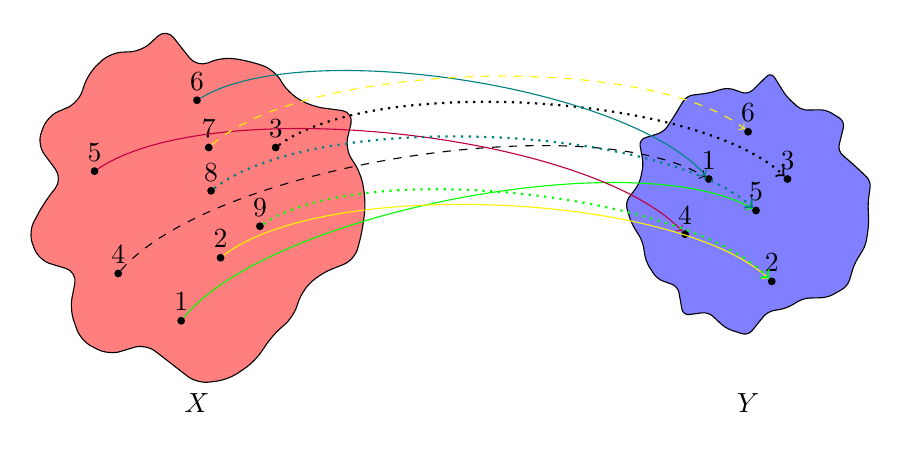
\begin{tikzpicture}
\node (a) at (0,0) {};
\filldraw[fill = red, fill opacity = .5, rounded corners=1.5mm] (a) \irregularcircle{2cm}{3mm};
\node (b) at (7,0) {};
\filldraw[fill = blue, fill opacity = .5, rounded corners=.8mm] (b) \irregularcircle{1.5cm}{2mm};
\node[circle, fill, scale = .3] (1) at (-.2,-1.5) {};
\node[above] (naa) at (-.2,-1.5) {1};
\node[circle, fill, scale = .3] (2) at (.3,-.7) {};
\node[above] (nab) at (.3,-.7) {2};
\node[circle, fill, scale = .3] (3) at (1,.7) {};
\node[above] (nac) at (1,.7) {3};
\node[circle, fill, scale = .3] (4) at (-1,-.9) {};
\node[above] (nad) at (-1,-.9) {4};
\node[circle, fill, scale = .3] (5) at (-1.3,.4) {};
\node[above] (nae) at (-1.3,.4) {5};
\node[circle, fill, scale = .3] (6) at (0,1.3) {};
\node[above] (naf) at (0,1.3) {6};
\node[circle, fill, scale = .3] (7) at (.15,.7) {};
\node[above] (nag) at (.15,.7) {7};
\node[circle, fill, scale = .3] (8) at (.18,.15) {};
\node[above] (nah) at (.18,.15) {8};
\node[circle, fill, scale = .3] (9) at (.8,-.3) {};
\node[above] (nai) at (.8,-.3) {9};
%
%
%
%
\node[circle, fill, scale = .3] (10) at (6.5, .3) {};
\node[above] (nba) at (6.5, .3) {1};
\node[circle, fill, scale = .3] (11) at (7.3, -1) {};
\node[above] (nbb) at (7.3, -1) {2};
\node[circle, fill, scale = .3] (12) at (7.5,.3) {};
\node[above] (nbb) at (7.5,.3) {3};
\node[circle, fill, scale = .3] (13) at (6.2,-.4) {};
\node[above] (nbb) at (6.2,-.4) {4};
\node[circle, fill, scale = .3] (14) at (7.1,-.1) {};
\node[above] (nbb) at (7.1,-.1) {5};
\node[circle, fill, scale = .3] (15) at (7, .9) {};
\node[above] (nbb) at (7, .9) {6};
%
%
%
%
\draw[->, green] (1) edge[bend left=40,looseness=.6] (14);
\draw[->, yellow] (2) edge[bend left=40,looseness=.6] (11);
\draw[->, thick, dotted] (3) edge[bend left=40,looseness=.6] (12);
\draw[->, dashed] (4) edge[bend left=40,looseness=.6] (10);
\draw[->, purple] (5) edge[bend left=40,looseness=.6] (13);
\draw[->, teal] (6) edge[bend left=40,looseness=.6] (10);
\draw[->, yellow, dashed] (7) edge[bend left=40,looseness=.6] (15);
\draw[->, teal, thick, dotted] (8) edge[bend left=40,looseness=.6] (14);
\draw[->, green, thick, dotted] (9) edge[bend left=40,looseness=.6] (11);
\node[below] at (0,-2.3) {$X$};
\node[below] at (7,-2.3) {$Y$};
\end{tikzpicture}
\caption{A surjection from $X$ to $Y$}
\end{figure}
Here, we have a function $f:X\mapsto Y$, with $X=\set{1,2,3,4,5,6,7,8,9}$, and $Y=\set{1,2,3,4,5,6}$, and 
\[f=\set{(1,5),(2,2),(3,3),(4,1),(5,4),(6,1),(7,6),(8,5),(9,2)}\]
Note that some second elements of ordered pairs are repeated!  
\begin{definition}[Injective Function]
A function \[f:X\mapsto Y\] is said to be \textbf{injective} (or \textbf{one-to-one}) if each $y\in \text{im }f$ is paired with \emph{exactly one} $x\in X$.  Equivalently stated, if we have $x_1,x_2\in X$, then 
\[f(x_1) = f(x_2) \iff x_1 = x_2\]
Note that this is \emph{not} the same as saying `each $y\in Y$ is paired with exactly one $x\in X$.'  $\text{im }f$ is not necessarily the same as $Y$.  An \textbf{injective} function is referred to as an \textbf{injection}.
\end{definition}
In this sense, in an \textbf{injective} function, no $y\in Y$ can be `hit' by the funciton more than once:
\begin{figure}[H]
\centering
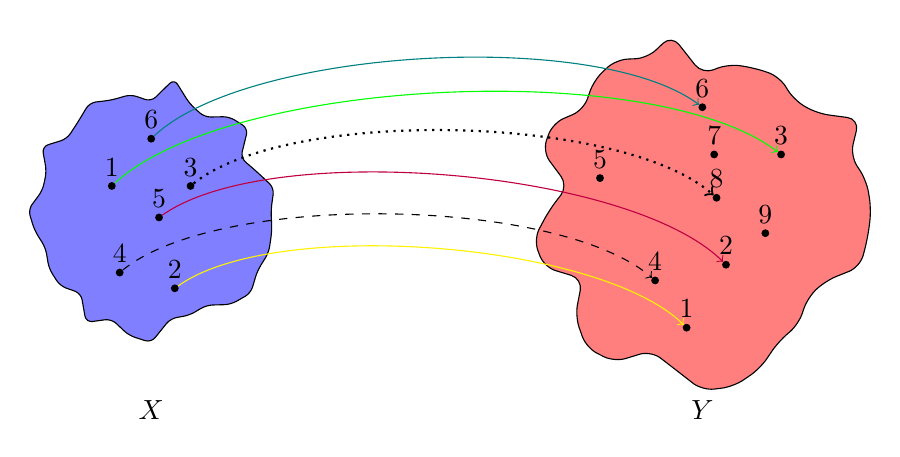
\begin{tikzpicture}
\node (a) at (7,0) {};
\filldraw[fill = red, fill opacity = .5, rounded corners=1.5mm] (a) \irregularcircle{2cm}{3mm};
\node (b) at (0,0) {};
\filldraw[fill = blue, fill opacity = .5, rounded corners=.8mm] (b) \irregularcircle{1.5cm}{2mm};
\node[circle, fill, scale = .3] (1) at (6.8,-1.5) {};
\node[above] (naa) at (6.8,-1.5) {1};
\node[circle, fill, scale = .3] (2) at (7.3,-.7) {};
\node[above] (nab) at (7.3,-.7) {2};
\node[circle, fill, scale = .3] (3) at (8,.7) {};
\node[above] (nac) at (8,.7) {3};
\node[circle, fill, scale = .3] (4) at (6.4,-.9) {};
\node[above] (nad) at (6.4,-.9) {4};
\node[circle, fill, scale = .3] (5) at (5.7,.4) {};
\node[above] (nae) at (5.7,.4) {5};
\node[circle, fill, scale = .3] (6) at (7,1.3) {};
\node[above] (naf) at (7,1.3) {6};
\node[circle, fill, scale = .3] (7) at (7.15,.7) {};
\node[above] (nag) at (7.15,.7) {7};
\node[circle, fill, scale = .3] (8) at (7.18,.15) {};
\node[above] (nah) at (7.18,.15) {8};
\node[circle, fill, scale = .3] (9) at (7.8,-.3) {};
\node[above] (nai) at (7.8,-.3) {9};
%
%
%
%
\node[circle, fill, scale = .3] (10) at (-.5, .3) {};
\node[above] (nba) at (-.5, .3) {1};
\node[circle, fill, scale = .3] (11) at (.3, -1) {};
\node[above] (nbb) at (.3, -1) {2};
\node[circle, fill, scale = .3] (12) at (.5,.3) {};
\node[above] (nbb) at (.5,.3) {3};
\node[circle, fill, scale = .3] (13) at (-.4,-.8) {};
\node[above] (nbb) at (-.4,-.8) {4};
\node[circle, fill, scale = .3] (14) at (.1,-.1) {};
\node[above] (nbb) at (.1,-.1) {5};
\node[circle, fill, scale = .3] (15) at (0, .9) {};
\node[above] (nbb) at (0, .9) {6};
%
%
%
%
\draw[->, green] (10) edge[bend left=40,looseness=.6] (3);
\draw[->, yellow] (11) edge[bend left=40,looseness=.6] (1);
\draw[->, thick, dotted] (12) edge[bend left=40,looseness=.6] (8);
\draw[->, dashed] (13) edge[bend left=40,looseness=.6] (4);
\draw[->, purple] (14) edge[bend left=40,looseness=.6] (2);
\draw[->, teal] (15) edge[bend left=40,looseness=.6] (6);
\node[below] at (0,-2.3) {$X$};
\node[below] at (7,-2.3) {$Y$};
%
%
%
%
\end{tikzpicture}
\caption{An injection from $X$ to $Y$}
\end{figure}
Here, we have a \textbf{injective} function $f:X\mapsto Y$ with $X=\set{1,2,3,4,5,6}$ and $Y=\set{1,2,3,4,5,6,7,8,9}$, 
\[f = \set{(1,3),(2,1),(3,8),(4,4),(5,2),(6,6)}\]
For the most part, this happens when $Y$ has more elements than $X$.\footnote{note that this doesn't mean that if $Y$ is bigger than $X$ then the function will be a surjection---the statement is that \emph{if} the function is a surjection, than most of the time $Y$ will have more elements than $X$.}  Note that in the example above, there are $y\in Y$ that are not in im $f$ (i.e., the function does not `hit' every element of $Y$).\\~\\
When a function is both $\textbf{injective}$ and $\textbf{surjective}$, we have a special name for it: a $\textbf{bijection}$.  
\begin{definition}[Bijection]
A \textbf{bijection} between two sets $X$ and $Y$ is a function $f:X\mapsto Y$ such that $f$ is both injective (one-to-one) and surjective (onto).  
\end{definition}  
So, for a bijection $f:X\mapsto Y$, we have $\text{im }f = Y$, and no $y\in Y$ appears as the second element in more than one ordered pair of our funciton (see if you can prove this).  Bijections can only occur if the domain and codomain have the same number of elements.  \\~\\
In my descriptions of surjections, injections, and bijections, I spoke loosely about the `usual' number of elements in the domain and codomain.  There is a surprisingly useful mathematical tool that formalizes these concepts, called the \textbf{pigeonhole principle}.  
\begin{theorem}[Pigeonhole Principle]
If $X$ and $Y$ are finite sets and we have a function $f:X\mapsto Y$, then 
\begin{enumerate}
    \item If $X$ has more elements than $Y$, $f$ is not one-to-one 
    \item If $X$ has fewere elements than $Y$, then $f$ is not onto. 
    \item If $f$ is a bijection, then $X$ and $Y$ have the same number of elements.  
\end{enumerate}
\end{theorem}
Here, we will not actually prove the pigeonhole principle, because I'm lazy.  As it turns out, the pigeonhole principle can be used to prove a remarkable number of non-obvious results.  However, notice the caveat in the theorem statement: $X$ and $Y$ \emph{must} be finite sets.  When we deal with infinite sets, the idea of the `number of elements' in a set begins to break down.  
% David Mollet, paintings are from up in the Brooks range
\begin{leftbar}[.95\linewidth]
\begin{enumerate}
    \item Show that $f:\NN \mapsto \ZZ$, given by 
    \begin{equation*}
    f(n) = 
    \begin{cases}
    -\frac{n}{2} & \text{if $n$ is even} \\ 
    \frac{(n+1)}{2} & \text{if $n$ is odd}
    \end{cases}
    \end{equation*}
    Is a bijection.  In this sense, we say that it makes sense to say that $\NN$ and $\ZZ$ have the `same number of elements,' because we can uniquely pair $n\in\NN$ with $z\in\ZZ$.  However, it can be shown that we can't form such a bijection between $\NN$ and $\RR$---in this sense, $\RR$ is `more infinite' than $\NN$ \emph{and} $\ZZ$!
    \item 
\end{enumerate}
\end{leftbar}
\subsection{Limits \& Continuity}
\end{document}
